\section{Multi-Level Computation Reuse}

This work has as its main goal the development of Sensitivity Analysis (SA) optimizations through multi-level computation reuse. This chapter analyzes computation reuse and then describes improvements made to the Region Templates Framework (RTF), which were implemented in order to enable the use of multi-level computation reuse. After that, the new computation reuse approaches are described, along with their advantages and disadvantages.

\begin{figure}[t]
\begin{center}
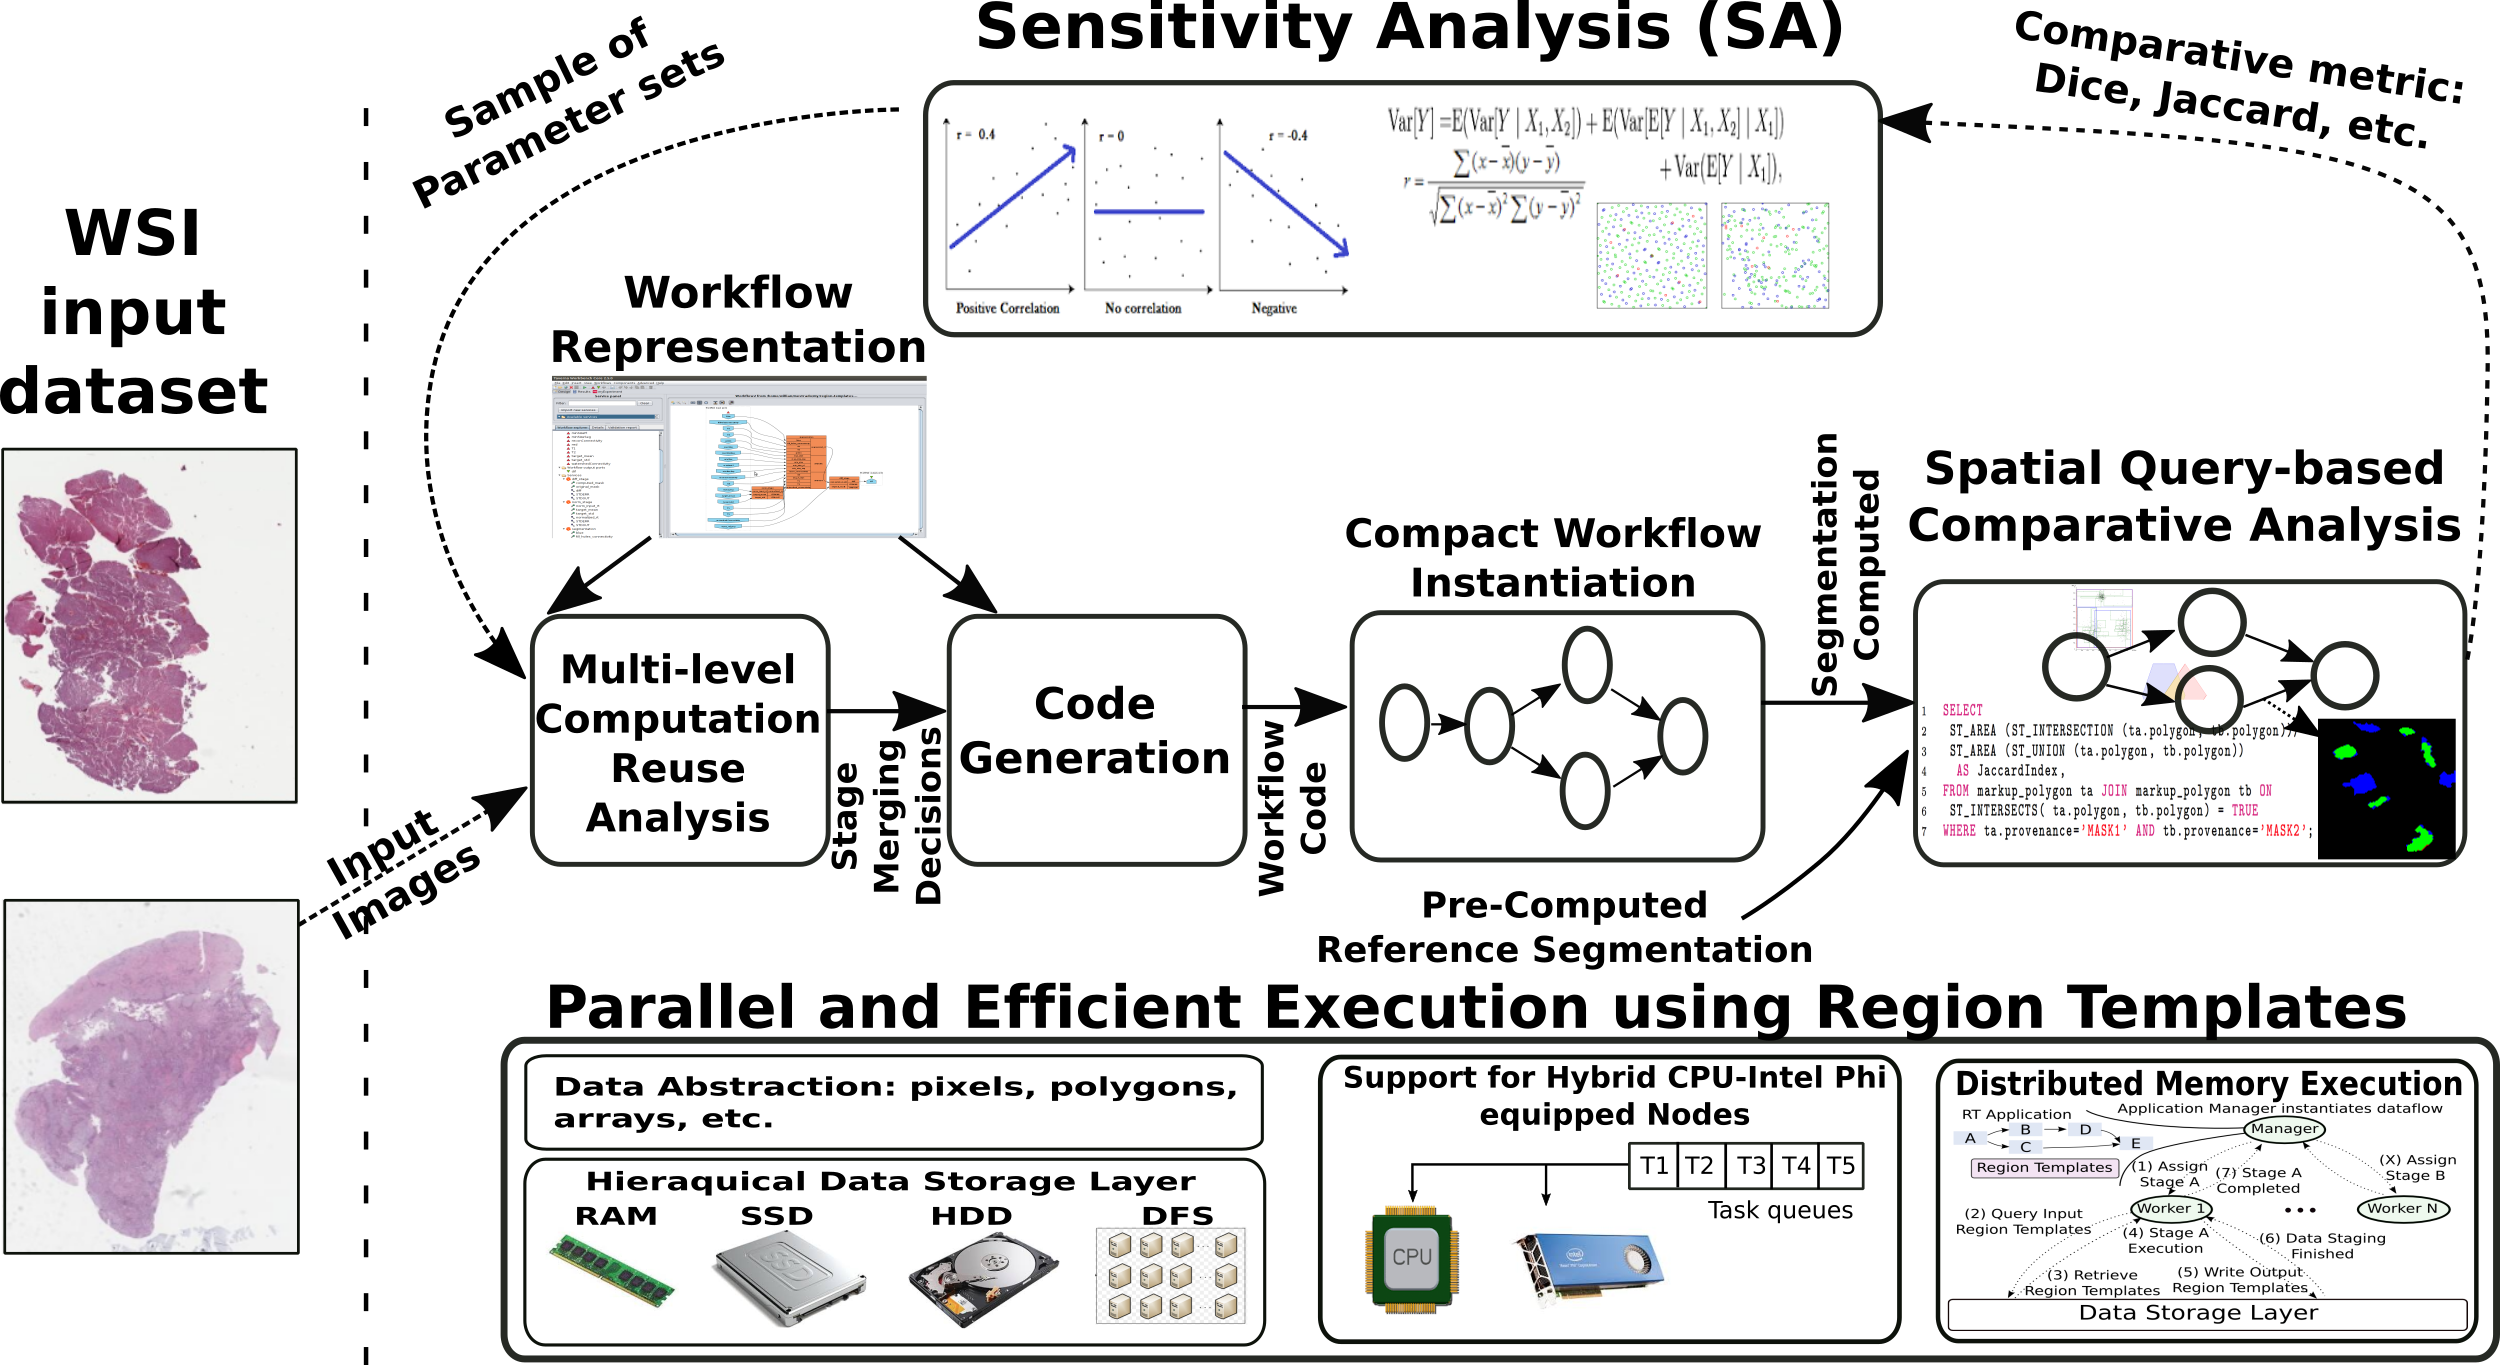
\includegraphics[width=0.7\textwidth]{img/functions.png} \caption{The parameter study framework. A SA method selects parameters of the analysis workflow, which is executed on a parallel machine. The workflow results are compared to a set of reference results to compute differences in the output. This process is repeated a set number of times (sample size) with varying input parameters' values.}
\label{fig:overview}
\end{center}
\vspace{-4mm}
\end{figure}

The SA studies and components that were developed and integrated into the RTF are illustrated in Figure \ref{fig:overview}. An SA study in this framework starts with the definition of a given workflow, the parameters to be studied, and the input data. The workflow is then instantiated and executed efficiently in RT using parameters values selected by the SA method. These values, or parameters sets, are generated separately by the user through a SA method statically, i.e, before the execution of any task on the RTF. The output of the workflow is compared using a metric selected by the user to measure the difference between a reference segmentation result and the one computed by the workflow using the parameter set generated by the SA method. This process continues while the number of workflow runs does not achieve the sample size required by the SA. This sample size is effectively the number of times that the workflow will be instantiated and executed with different input parameters' values. The sample size is a way to limit the cost of the SA study while maintaining its significance and accuracy. This can be done by empirically choosing a sample size that is big enough to have accurate results but not enough that its cost is unfordable.

\begin{figure}[b!]
\begin{center}
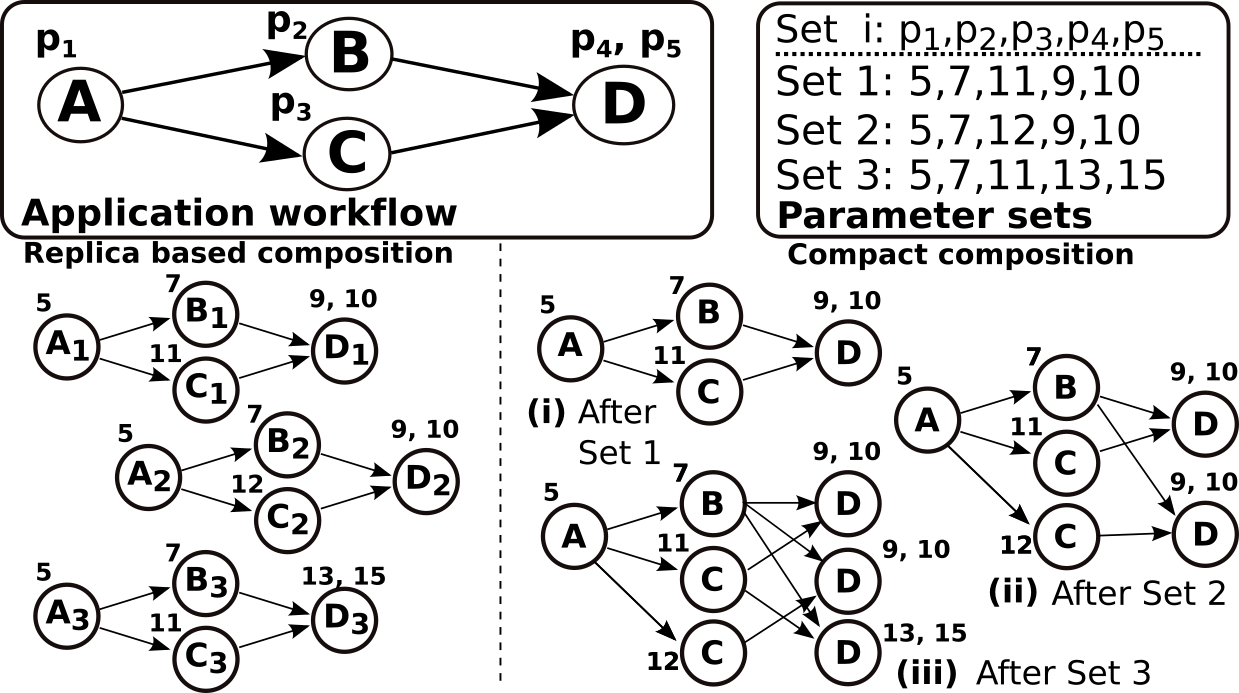
\includegraphics[width=0.8\textwidth]{img/reuse.png}
\caption{A comparison of a workflow generated with and without computation reuse. Image extracted from \cite{rtf2}.}
\label{fig:reuse}
\end{center}
\vspace{-4mm}
\end{figure}

Computation reuse is achieved through the removal of repeated computation tasks. Figure \ref{fig:reuse} presents the comparison of a replica-based workflow generation, in which there is no reuse, and a compact composition, generated with maximal reuse. Given that we start generating a compact composition with no tasks on it, the first parameter set (Set 1, (i) in Figure \ref{fig:reuse}) is added to the workflow in its entirety (i.e., all computation tasks A-D). The second parameter set, however, has the reuse opportunities of tasks A and B given they have the same input parameters values and input data. Thus, only the tasks C and D for parameter set 2 are instantiated in the compact graph ((ii) in Figure \ref{fig:reuse}). With the current workflow state of (ii), parameter set 3 presents reuse opportunities for tasks A, B and C, thus only needing to instantiate a single computation task (D) with the parameters values 13 and 15 to the workflow. When comparing the workflow replica based composition with the compact composition we can notice a decrease on the number of executed tasks of approximately 41\%, from 12 tasks to 7 tasks.

There are two computation reuse levels used on this work, (i) stage-level, on which coarse-grain computation tasks are reused, and (ii) task-level - with fine-grain tasks reused. Coarse-grain computation reuse is significantly easier to implement than its fine-grained counterpart. However, the number of parameters that two coarse-grained merging candidates stages need to match for the reuse to take place is higher as when compared with fine-grain tasks.




\subsection{Graphical User Interface and Code Generator}
\label{sec:improve}

In this work a flexible task-based stage code generator was implemented to ease the process of developing RTF applications. This generator was created, together with a workflow generator graphical interface - with the purpose of making the RTF more accessible to domain-specific experts. Additionally, this code generator will simplify the application information gathering process, necessary for merging stages instances during the process of computation reuse.

\begin{figure}[h!]
\vspace{-4mm}
\begin{center}
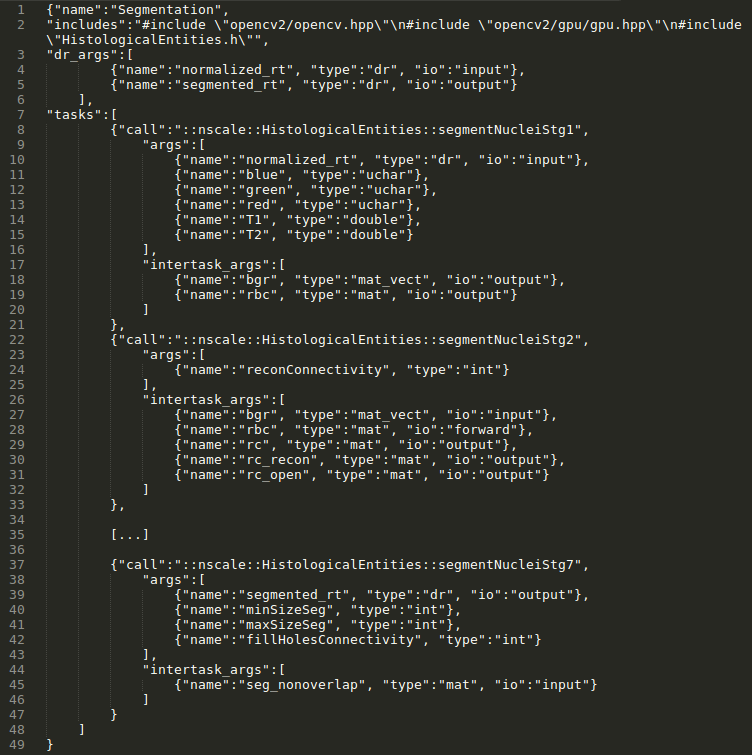
\includegraphics[width=0.6\textwidth]{img/stage_gen.png}
\caption{An example stage descriptor Json file.}
\label{fig:cgen}
\end{center}
\vspace{-4mm}
\end{figure}

The stage generator has as its input a stage descriptor file, formatted as Json, as shown in Figure \ref{fig:cgen}. A stage is defined by its name, the external libraries it needs to call in order to execute the application domain transformations in each stage of the workflows, the necessary input arguments for its execution and the tasks it must execute. There are two kinds of inputs: the arguments and the Region Templates (RT). The arguments are constant inputs, which are varied by the given SA method and represent the application input parameter values. The RT is the data structure provided by the RTF for inter-stage and inter-task communication. As seen on the example descriptor file, only the RT inputs are explicitly written, while the remaining arguments can be inferred from the tasks descriptions.

Every stage is comprised of tasks, described by (i) the external call to the library of operations implemented by the user and (ii) its arguments. On Figure \ref{fig:cgen} the call for the first task is \textit{segmentNucleiStg1} from the external library \textit{nscale}. The arguments can be one of two types, (i) constant input arguments (args), defined by the SA application or (ii) intertask arguments (intertask\_args), which are produced/consumed for/by a fine-grain task.

\begin{figure}[h!]
\begin{center}
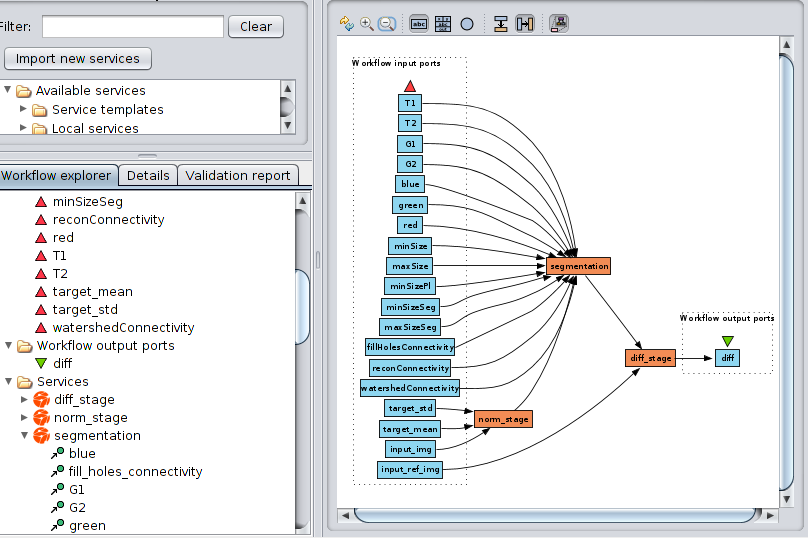
\includegraphics[width=0.8\textwidth]{img/taverna.png}
\caption{The example workflow described with the Taverna Workbench.}
\label{fig:tav1}
\end{center}
\vspace{-4mm}
\end{figure}

With task-based stages generated, the user can instantiate workflows using the newly generated stages. As with tasks, the RTF did not support a flexible, non-compiled solution for generating workflows, being these workflows hardcoded into the RTF. The solution implemented on this work was to use the Taverna Workbench tool \cite{taverna} as a graphical interface for producing workflows and implement a parser for the generated Taverna file. An example workflow on the Taverna Workbench is displayed on Figure \ref{fig:tav1}.

\subsection{Stage-Level Merging}
\label{sec:stage-merging}

The stage level merging needs to identify and remove common stage instances and build a compact representation of the workflow, as presented in Algorithm~\ref{alg:stg-merg}. The algorithm receives the application directed workflow graph (appGraph) and parameter sets to be tested as input (parSets) and outputs the compact graph (comGraph). It iterates over each parameter set (lines 3-5) to instantiate a replica of the application workflow graph with parameters from $set$. It then calls {\scshape MergeGraph} to merge the replica to the compact representation.  

\begin{algorithm}[b!]
\small
	\caption{Compact Graph Construction
	\label{alg:stg-merg}}
		
	\begin{algorithmic}[1]
	\State {\bf Input:} appGraph; parSets;
	\State{\bf Output:} comGraph;
	\For{{\bf each} set $\in$ parSets}
		\State appGraphInst = \Call{instantiateAppGraph}{set};
		\State \Call{MergeGraph}{appGraphInst.root, comGraph.root};
	\EndFor
	\Procedure{MergeGraph}{appVer, comVer}
		\For{{\bf each} v $\in$ appVer.children}
			\If{(v' $\gets$ find(v, comVer.children))}
				\State \Call{MergeGraph}{v, v'};
			\Else
				\If{((v' $\gets$ PendingVer.find(v))==$\emptyset$)}
					\State v' $\gets$ clone(v)
					\State v'.depsSolved $\gets$ 1
					\State comVer.children.add(v')
					\If{v'.deps $\ge$ 1}
						\State PendingVer.insert(v')
					\EndIf
					\State \Call{MergeGraph}{v, v'};
				\Else
					\State comVer.children.add(v')
					\State v'.depsSolved $\gets$ v'.depsSolved+1
					\If{v'.depsSolved == v'.deps}
						\State PendingVer.remove(v')
					\EndIf
					\State \Call{MergeGraph}{v, v'}
				\EndIf
			\EndIf    
		\EndFor
	\EndProcedure
	\end{algorithmic}
\end{algorithm}

The {\scshape MergeGraph} procedure walks simultaneously in an application workflow graph instance and in the compact representation. If a path in the application workflow graph instance is not found in the latter, it is added to the compact graph.  The {\scshape MergeGraph} procedure receives the current set of vertices in the application workflow ($appVer$) and in the compact graph ($comVer$) as a parameter and, for each child vertex of the $appVer$, finds a corresponding vertex in the children of $comVer$. Each vertex in the graph has a property called {\em deps}, which refers to its number of dependencies. The find step considers the name of a stage and the parameters used by the stage. If a vertex is found, the path already exists, and the same procedure is called recursively to merge sub-graphs starting with the matched vertices (lines 9-10). When a corresponding vertex is not found in the compact graph, there are two cases to be considered (lines 11-26). In the first one, the searched node does not exist in $comGraph$. The node is created and added to the compact graph (lines 12-18). To check if this is the case, the algorithm verifies if the node ($v$) has not been already created and added to $comGraph$ as a result of processing another path of the application workflow that leads to $v$. This occurs for nodes with multiple dependencies, e.g., D in Figure~\ref{fig:reuse}. If the path (A,B,D) is first merged to the compact graph, when C is processed, it should not create another instance of D. Instead, the existing one should be added to the children list as the algorithm does in the second case (lines 21-25). The $PendingVer$ data structure is used as a look-up table to store such nodes with multiple dependencies during graph merging. This algorithm makes $k$ calls to {\scshape MergeGraph} for each $appGraphInst$ to be merged, where $k$ is the number of stages of the workflow. The cost of each call is dominated by the $find$ operation in the $comVer.children$. The $children$ will have a size of up to $n$ or $|parSets|$ in the worst case. By using a hash table to implement children, the find is $\mathcal{O}$($1$). Thus, the insertion of $n$ instances of the workflow in the compact graph is $\mathcal{O}$($kn$).



\subsection{Task-Level Merging}

On the previous section coarse-grain reuse was implemented through a stage-level merging algorithm. This approach can by itself attain good speedups for the workflow used on this work. However, due to the granularity of the stages there is still many reuse opportunities which are wasted since they are not visible or even achievable on stage-level. These opportunities are visible though on task-level, through what we define as fine-grain reuse. This reuse can be achieved by merging stages together and removing the repeated tasks, through what we call task-level merging. Merging at task-level, unlike stage-level, has some limitations due to the way stages and tasks are implemented on the RTF. Tasks are a finer-grain computational job, intended to be small activities. Although stages can be executed on distinct computing nodes, tasks cannot, since it would not make sense to distribute such small tasks which communication overhead over the nodes network would most likely outweigh the task cost itself.

With these peculiarities in mind, before we implement any fine-grain merging algorithm we must first address some limitations on excessive fine-grain reuse. When excessive task-level merging is performed the joint number of parameters and variables of a merged stage, containing a large number of tasks, may not fit on the system memory. These variables are most of the times intermediate data that is passed between tasks, also including intermediate images, which are rather large for the purpose of this work. Also, it is possible for all stages to be merged in a number smaller than the number of available nodes, hence making some of the available resources idle. Both these problems can be solved by limiting the maximum number of stages that can be merged (bucket size). This limit is defined here as $MaxBucketSize$. Another way to enforce memory restriction is to limit the maximum number of tasks per group of merged stages (buckets). This limit is the $MaxBuckets$.

\subsubsection{Na\"ive Algorithm}
\label{sec:naive-merging}

In the interest of better understanding the task-level merging problem, a na\"ive algorithm was implemented to serve as a baseline for our analysis. This simplified algorithm groups $MaxBucketSize$ stages in buckets and attempts to merge all stages of each bucket among themselves. This was achieved by sequentially grouping the first $MaxBucketSize$ stages into buckets, until there are no more stages to be merged. 

%The $MaxBucketSize$ constraint was employed as a mechanism to prevent the generation of merged stages that are impossible to execute. This can happen if a bucket is big enough such that a node could not hold all the stages running concurrently (not enough memory for all arguments). We recognize that this value is of such importance that further work will be conducted to find ways to optimize it.

Although this simple solution was quickly implemented and has a linear algorithmic complexity its reuse efficiency is, however, highly dependent on the stages ordering. For instance, if similar stages were to be generated close together a greater amount of reusable computation is more likely to exist.


\subsubsection{Smart Cut Algorithm (SCA)}
\label{sec:sca}

Another strategy to create buckets of stages to be merged that was investigated is through the use of a graph based representation (see Figure \ref{fig:sca}). A representation for this could be done using fully-connected undirected graphs on which the stage instances are the nodes and each edge is the degree of reuse between two stage instances (Figure \ref{fig:sca1}). By degree of reuse we mean the number of tasks that would be reused if the two stages are merged. With this perspective we would need only to partition this graph in subgraphs, maximizing the reuse degree of all subgraphs. This is a well-known problem, called min-cut \cite{mincut}. 

\begin{figure}[!h]
	 \centering
	 \begin{subfigure}[b]{0.3\textwidth}
			\centering
			 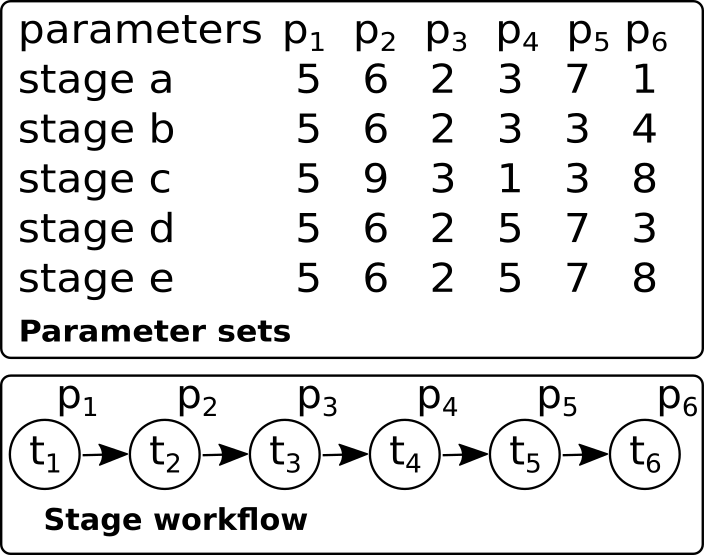
\includegraphics[width=\textwidth]{img/sca0.png}
			 \caption{Example application.}
			 \label{fig:sca0}
	 \end{subfigure}
	 \hspace{3mm}
	 \begin{subfigure}[b]{0.3\textwidth}
			\centering
			 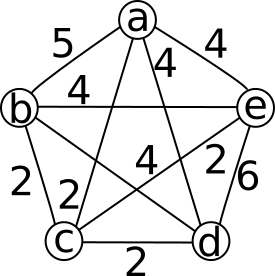
\includegraphics[width=\textwidth]{img/sca1.png}
			 \caption{Initial graph of instance example.}
			 \label{fig:sca1}
	 \end{subfigure}
	 \hspace{3mm}
	 \begin{subfigure}[b]{0.3\textwidth}
			 \centering
			 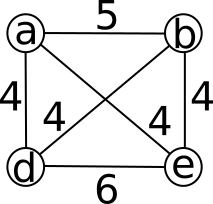
\includegraphics[width=0.8\textwidth]{img/sca2.png}
			 \caption{First cut is performed, removing node $c$.}
			 \label{fig:sca2}
	 \end{subfigure}
	 \par\bigskip
	 \begin{subfigure}[b]{0.3\textwidth}
			 \centering
			 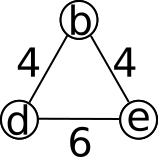
\includegraphics[width=0.8\textwidth]{img/sca3.png}
			 \caption{After the next cut node $a$ is removed.}
			 \label{fig:sca3}
	 \end{subfigure}
	 \hspace{3mm}
	 \begin{subfigure}[b]{0.3\textwidth}
			 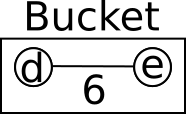
\includegraphics[width=0.8\textwidth]{img/sca4.png}
			 \centering
			 \caption{After final cut of node $b$ $MaxBucketSize$ sized subgraph is found.}
			 \label{fig:sca4}
	 \end{subfigure}
	 \hspace{3mm}
	 \begin{subfigure}[b]{0.25\textwidth}
			 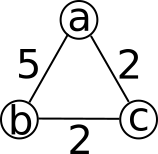
\includegraphics[width=\textwidth]{img/sca5.png}
			 \caption{The cutting starts over with the remaining nodes.}
			 \label{fig:sca5}
	 \end{subfigure}
	 
		\caption{An example on which SCA executes on 5 instances of a workflow application of 6 tasks, with $MaxBucketSize = 2$.}
		\label{fig:sca}
\end{figure}

Although there are many variations for the min-cut problem \cite{mincut,minkcut}, we define here a min-cut algorithm as one that takes an undirected graph and performs a 2-cut (i.e., cut the graph in two subgraphs) operation, minimizing the sum of the cut edges weight. This 2-cut operation was selected because of its flexibility and computational complexity. First, the recursive use of 2-cuts can break a graph in any number of subgraphs. Moreover, k-cut algorithms are not only more computationally intensive than 2-cut algorithms, but also have no guarantees for the balancing of the subgraphs (e.g., for $k=5$ on a graph with 10 nodes one possible solution is 4 subgraphs with 1 node each and 1 subgraph with 6 nodes). As such, we can implement a simple k-cut balanced algorithm by performing 2-cut operations on the most expensive graph/subgraph until a stopping condition is reached (e.g., number of subgraphs is reached, number of nodes per subgraph is reached). With all these considerations only 2-cut operations are used on the proposed algorithm.

Figure \ref{fig:sca} demonstrates a way to group stages into buckets using 2-cut operations. First, the fully-connected graph in Figure \ref{fig:sca1} is generated given the stage instances of Figure \ref{fig:sca0}. Figure \ref{fig:sca2} shows the result of the first 2-cut operation, on which the subgraph containing only the node $c$ is found to be the one least related to the subgraph with the remaining nodes. This is similar to the state that $c$ is the ``least reusable'' stage among all other stages (i.e., the stage which, if selected for merging, would have highest computational cost). Next, nodes $a$ and $b$ are removed until a bucket of size 2 is reached (see Figures \ref{fig:sca2} and \ref{fig:sca3}). The previously removed nodes ($a$, $b$ and $c$) are then put together (Figure \ref{fig:sca5}) and the same cutting algorithm starts over. This process is then repeated until all stages are grouped into buckets.

% An alternative was to employ a k-cut algorithm, however, the sole minimization of the cut could result in an unbalanced solution. For instance, lets say we want $k$ buckets for $n$ stages and there are $k$ unmergeable stages, and that one of the $k$ unmergeable is can be merged with the remaining $n-k$ stages. The solution for this instance would be $k-1$ buckets with a single stage and one bucket with $n-k+1$ stages, which would in turn result in performance degradation.

% In favor of producing balanced solutions a fully-recursive approach was implemented, on which each set of stages $s$ would be 2-cut into $s1$ and $s2$, with $|s1| \geq |s2|$. Both $s1$ and $s2$ would go through the same 2-cut process until their size would come to be less or equal to $MaxBucketSize$. At the end of this recursive process a solution would be found. In order to find other solutions, $s1$ would be 2-cut again, into $s1'$ and $s1''$, being $|s1'| \geq |s1''|$, $s1'$ would become the new $s1$ and $s1''$ would merge with $s2$. From this point the recursion would restart for the new $s1$ and $s2$. This backtracking routine would go as long as the new solution is better than the last one, for it's believed that it's impossible to find a better solution $sol_b$ after the solution $sol$ is found, and then the worse solution $sol'$ is found. If this statement is true this algorithm returns the best global solution. However, the amount of time needed for its completion makes this approach unfeasible, being this an superpolynomial algorithm.

% A second attempt made was to use a Monte-Carlo approach on the recursion of $s1$ and $s2$, thus attenuating the almost exponential behavior of the algorithm. Nonetheless, this approach produced significantly worse solutions, being them highly unbalanced. This occurred because a partial solution on a higher level of the 2-cut process would have such a huge impact on the final solution, and this first partial solution would hardly be a good one on account for the Monte-Carlo process.

With this procedure in mind Algorithm \ref{alg:scut} was designed. 
This algorithm performs successive 2-cut operations on the graphs to divide it into
disconnected subgraphs that fit in a bucket. The cuts are performed such that
the amount of reuse lost with a cut is minimized. In more detail, the partition
process starts by dividing the graph into 2 subgraphs (s1 and s2) using a minimum cut
algorithm~\cite{mincut} (line 4). Still, after the cut, both
subgraphs may have more than $MaxBucketSize$ vertices. In this case, another
cut is applied in the subgraph with the largest number of stages (lines 5-7), and this is
repeated until a viable subgraph (number of stages $\leq$ $MaxBucketSize$) is
found.  When this occurs, the viable subgraph is removed from the original
graph (lines 8-11), and the full process is repeated until the graphs with stage instances
yet not assigned to a bucket can fit in one.

\begin{algorithm}[t!]
\small
	\caption{Smart Cut Algorithm
		\label{alg:scut}}
				
	\begin{algorithmic}[1]
		\State {\bf Input:} stages; MaxBucketSize;
	\State{\bf Output:} bucketList;
		
		\While{|stages| > 0}
			\State \{s1,s2\} $\gets$ \Call{2cut}{stages}
				\While{|s1| > MaxBucketSize}
					\State \{s1,s2\} $\gets$ \Call{2cut}{s1}
				\EndWhile
				\State bucketList.add(s1)
				\For{{\bf each} s $\in$ s1}
					\State stages.remove(s)
				\EndFor
		\EndWhile
	\end{algorithmic}
\end{algorithm}

The number of cuts necessary to compute a single viable subgraph of $n$ stages is $\mathcal{O}$($n$) in the worst case. This occurs when each cut returns a subgraph with only one stage and another subgraph with the remaining nodes. The cut then needs to be recomputed -- about $n-MaxBucketSize)$ times -- on the largest subgraph until a viable subgraph is found. Also, in the worst case, all viable subgraphs would have $MaxBucketSize$ stages and, as such, up to $n/MaxBucketSize$ buckets could be created. Therefore, the algorithm will perform $\mathcal{O}$($n^2$) cuts in the worst case to create all buckets. In our implementation, the min-cut is computed using a Fibonacci heap~\cite{mincut} to speed up the algorithm, making each cut $\mathcal{O}$($E+V\ log\ V$). Since the graph used is fully connected, the complexity of a single cut in our case is $\mathcal{O}$($n^2$) and, as consequence, the full SCA is $\mathcal{O}$($n^4$).  Although the SCA computes good reuse solutions, its use in practice is limited because of the computational complexity.  This motivated the proposal of the strategy described in Section \ref{sec:rtma}.


% The third and final attempt at a 2-cut-based merging algorithm was to remove completely the recursion and focus on performing a better job at the first levels of partial solutions, named Smart Cut Algorithm (SCA), as described on Algorithm \ref{alg:scut}. This new algorithm consists on performing a 2-cut operation on the input stage list (stages), resulting in $s1$ and $s2$, with $|s1| \geq |s2|$, setting $s \gets s1$, and iterating through this process until $|s1| \leq MaxBucketSize$ (line 5). At this point $s1$ is set as a final solution bucket (line 8) and the same search process for a new bucket restarts with the remaining stages (lines 9-11).

% The number of cuts necessary to compute a single viable bucket is $\mathcal{O}$($n$), since on the worst case, each cut will only remove one stage from $s1$ (line 6), resulting in $n-MaxBucketSize$ cuts. This process is done $n/MaxBucketSize$ times, which is $\mathcal{O}$($n$), resulting in a final complexity of $\mathcal{O}$($n^2$) cut operations. In this work the cut algorithm was implemented using a Fibonacci Heap, as proposed by \textbf{[2cut algorithm ref]}, running in $\mathcal{O}$($E+V\ log\ V$) time. Since the graph fed to the 2-cut algorithm is fully-connected we have that the 2-cut algorithm runs in $\mathcal{O}$($n^2$) time. As a consequence the SCA is $\mathcal{O}$($n^4$).

% Although the solutions produced by the SCA are good and its runtime is of polynomial order of complexity, a $\mathcal{O}$($n^4$) algorithm is very expensive. Thus, it was expected that this approach wouldn't scale as it's necessary.



\subsubsection{Reuse Tree Merging Algorithm (RTMA)}
\label{sec:rtma}

Still on graphs, a natural way to display hierarchical structures is with trees. Using tasks as nodes on this tree, subtrees with the same parent node indicates that all child task nodes of said parent node use its output. As such, if we constructed a tree with several stages, we are able to easily see the reuse opportunities, lying in the nodes with more than one child node. Moreover, each level of the tree would represent a given task, which can be instantiated with different parameters sets. 

Detailing this structure, each level of the tree represents a task, and if a stage $s$ shares a parent node on level $k$ with $s'$, this implies that all tasks from 1 to $k$ are the same for both stages, an thus reusable among themselves (i.e., same computational task with the same inputs). This structure is defined as a Reuse Tree, with every node being defined by its level (or height), its parent, its children and a reference to the stage responsible for its generation.

\paragraph{Reuse-Tree Generation}

On a SA example we have a workflow $w$ that is instantiated $n$ times with different parameters ($w_1$, $w_2$, ..., $w_n$). Each workflow $w_i$ is composed by $m$ stages $s_{ij}$ with $i \in [1,n]$ and $j \in [1,m]$. A reuse-tree is then generated for each $j$-th stage level. The reuse-tree for a given stage level can be generated by iteratively inserting one stage instance after the other on the reuse-tree. Initially, a stage is represented as a tree on which every node has a single child and each node represents a task instantiation for that stage. Furthermore, any given node has as its parent a task that it is dependent on. Every stage is inserted one task node at a time. If, for a given task node, there already exists on the tree another node representing the same task with the same parameter inputs, said task node is not created, but instead the insertion process carries on from the equivalent node, characterizing task reuse.

\begin{figure}[h]
	 \centering
	 \begin{subfigure}[b]{0.3\textwidth}
			\centering
			 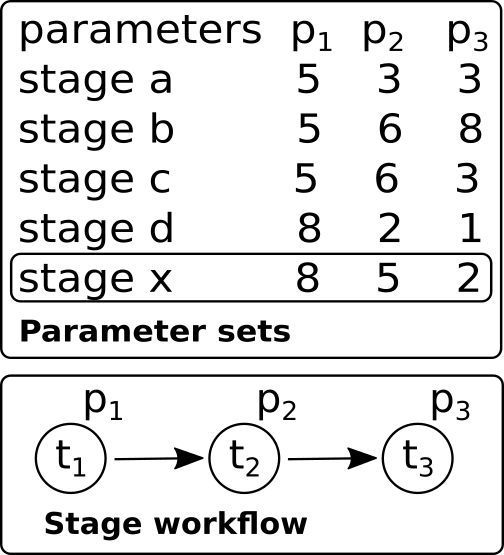
\includegraphics[width=\textwidth]{img/gen1-v2.png}
			 \caption{Example application.}
			 \label{fig:gen1}
	 \end{subfigure}
	 \hspace{3mm}
	 \begin{subfigure}[b]{0.3\textwidth}
			 \centering
			 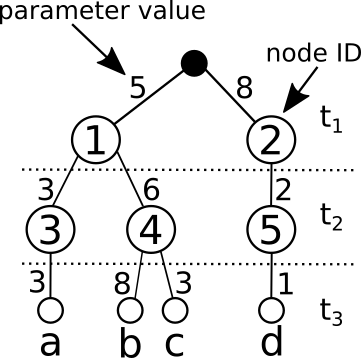
\includegraphics[width=0.8\textwidth]{img/gen2.png}
			 \caption{Initial reuse tree for the instance example.}
			 \label{fig:gen2}
	 \end{subfigure}
	 \hspace{3mm}
	 \begin{subfigure}[b]{0.3\textwidth}
			 \centering
			 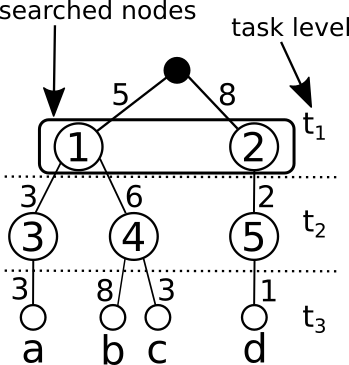
\includegraphics[width=0.8\textwidth]{img/gen3.png}
			 \caption{Searching for reuse on the first task.}
			 \label{fig:gen3}
	 \end{subfigure}
	 \par\bigskip
	 \begin{subfigure}[b]{0.3\textwidth}
			 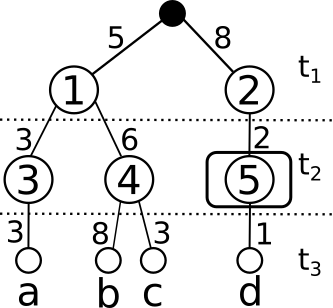
\includegraphics[width=0.8\textwidth]{img/gen4.png}
			 \centering
			 \caption{Searching for reuse on the second task.}
			 \label{fig:gen4}
	 \end{subfigure}
	 \hspace{3mm}
	 \begin{subfigure}[b]{0.3\textwidth}
			 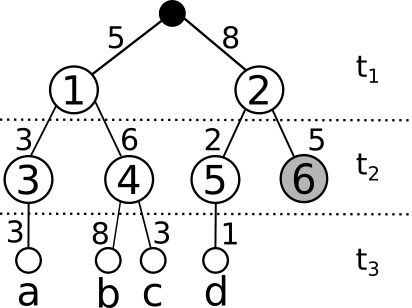
\includegraphics[width=\textwidth]{img/gen5.png}
			 \caption{Inserting a new node, 6.}
			 \label{fig:gen5}
	 \end{subfigure}
	 \hspace{3mm}
	 \begin{subfigure}[b]{0.3\textwidth}
			 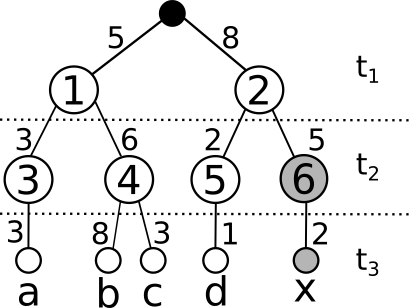
\includegraphics[width=\textwidth]{img/gen6.png}
			 \caption{Inserting the leaf node $x$.}
			 \label{fig:gen6}
	 \end{subfigure}
	 
		\caption{An example where node $x$ is inserted on the existing reuse tree. Figure \ref{fig:gen1} defines the tasks of which each stage is composed by and presents the parameters' values for each stage instance.}
		\label{fig:gen-ex}
\end{figure}

As an example, Figure \ref{fig:gen-ex} demonstrates the insertion of a stage (stage $x$) with the stage workflow and the parameters of each stage instance defined in Figure \ref{fig:gen1}, and the starting reuse tree in Figure \ref{fig:gen2}. Starting at the root node, its children (1 and 2) are searched for reuse opportunities for the first task (Figure \ref{fig:gen3}). Since node 2 represents all stages whose task 1 has as its input $p_1 = 8$ the first task of $x$ can be reused through it. The search for reuse of the second task is then performed on the children of node 2 (Figure \ref{fig:gen4}). Since node's 2 only child, node 5, cannot be reused for stage $x$'s second task (values for $p_2$ of stages $d$ and $x$ are different), a new node representing this non-reusable task is created (node 6) as shown in Figure \ref{fig:gen5}. Finally, since node 6 is new, there are no more reuse opportunities from it, thereby, a single child node must be created for each of the remaining non-reusable tasks (Figure \ref{fig:gen6}).

% The Reuse Tree generation is performed by successively adding new stages to the tree (line 4-6). The insertion starts at the root level (i.e., $0$). If the new stage (stage) has a reusable task on the current level (height) with at least one other previously added stage (lines 12-16) the found stage (reusableNode) is used to further the search for more reuse (line 23). If no stage with a reusable task of the current level (line 17) a new subtree for the current stage (stage) will be generated (lines 18-21). When the search for reuse/generation reaches the leaf level (line 8) the recursion ends, and with it the stage insertion procedure.

% Given the impractical solution that the SCA could be an entirely new approach was developed, having in mind the cost of merging. This final approach wouldn't have any of the high cost characteristics of the previous approaches, full recursion and 2-cut. 

% A different way of displaying the stages is in a tree structure, on which each level of the tree represents a task, and a stage $s$ that shares a parent node on level $k$ with $s'$ implies that all tasks from 1 to $k$ are reusable between both stages. This structure is defined as a Reuse Tree and its generation is described in Algorithm \ref{alg:rt-gen}. Any node on the Reuse Tree is defined by its level (or height), its parent, its children and a reference to the stage responsible for its generation.

% \begin{algorithm}
% \small
%   \caption{Reuse Tree Generator
%     \label{alg:rt-gen}}
				
%   \begin{algorithmic}[1]
%     \State {\bf Input:} stages;
%   \State{\bf Output:} reuseTree;
		
%     \State reuseTree.height $\gets$ N\textsuperscript{\underline{o}} of tasks per stage

%     \For{{\bf each} s $\in$ stages}
%       \State \Call{RecInsertStage}{reuseTree.parents, s, $\emptyset$, reuseTree.height, 0}
%     \EndFor
		
%     \Procedure{RecInsertStage}{nodeList, stage, parent, height, currLevel}
%     \If{(currLevel $=$ height)}
%       \State \Return
%     \EndIf

%     \State reusableNode $\gets$ $\emptyset$

%     \For{{\bf each} n $\in$ nodeList}
%       \If{(\Call{Reusable}{stage.tasks[height], n.stage.tasks[height]})}
%         \State reusableNode $\gets$ n
%       \EndIf
%     \EndFor

%     \If{(reusableNode $=$ $\emptyset$)}
%       \State newNode.parent $\gets$ parent
%       \State newNode.stage $\gets$ stage
%       \State nodeList $\gets$ [newNode$|$nodeList]
%       \State \Call{RecInsertStage}{newNode.children, stage, newNode, height, currLevel+1}
%     \Else
%       \State \Call{RecInsertStage}{reusableNode.children, stage, reusableNode, height, currLevel+1}
%     \EndIf
%   \EndProcedure

%   \end{algorithmic}
% \end{algorithm}

% \begin{figure}[htb!]
% \begin{center}
% \includegraphics[width=0.9\textwidth]{img/reuse-graphs.png}
% \caption{An example of Reuse Tree based merging with MaxBucketSize 3.}
% \label{fig:rt-example}
% \end{center}
% \end{figure}

\paragraph{The Merging Implementation}

In order for a merging algorithm to be implemented on top of the Reuse Tree structure we must take advantage of its hierarchical characteristics. Given that we want to bundle together buckets of stages of exactly $MaxBucketSize$ stages we must start with the deepest stages and move up. Figure \ref{fig:rg1} shows an example of a Reuse Tree with 12 stages and 3 tasks each. Stages $a$, $b$ and $c$ have two out of three reusable tasks, and as such, given a $MaxBucketSize=3$, should be put together in the same bucket. Meanwhile, stages $d$ through $i$ have one out of three reusable tasks. To maximize the reuse, stages $d$, $e$, $f$ and $g$ should be together, as should stages $h$ and $i$. Since $MaxBucketSize=3$, only 3 stages out of $d$, $e$, $f$ and $g$ can be put together, not mattering which 3 stages. This merger is seen in Figure \ref{fig:rg2}. After the merger of $d$, $e$ and $f$, stage $g$ is left alone, having as its best option, reuse-wise, to be put together with $h$ and $i$. As such, it is visible that the merging should happen in a bottom-up fashion.

\begin{figure}[!h]
	 \centering
	 \begin{subfigure}[b]{0.45\textwidth}
			 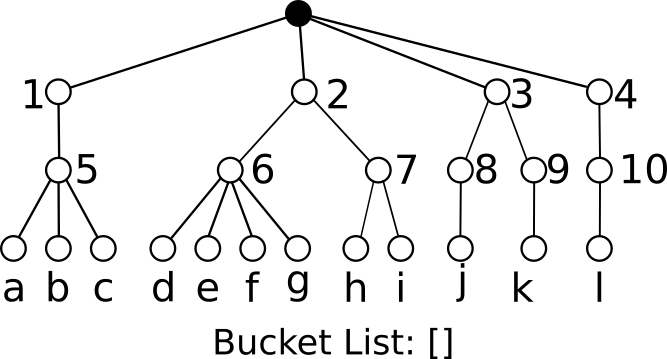
\includegraphics[width=\textwidth]{img/rg1.png}
			 \caption{Initial reuse tree.}
			 \label{fig:rg1}
	 \end{subfigure}
	 \hspace{3mm}
	 \begin{subfigure}[b]{0.45\textwidth}
				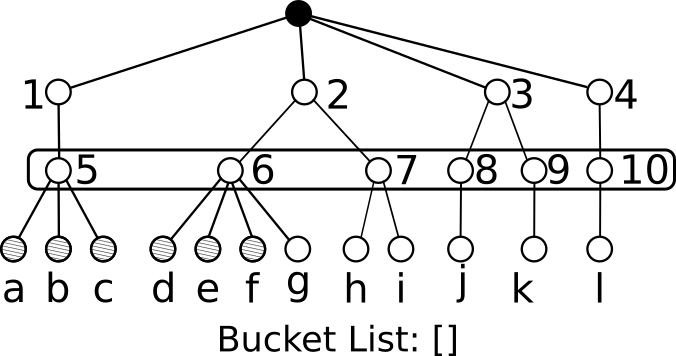
\includegraphics[width=\textwidth]{img/rg2.png}
				\caption{Reuse Tree after select procedure.}
				\label{fig:rg2}
		\end{subfigure}
		\par\bigskip
			 \begin{subfigure}[b]{0.45\textwidth}
				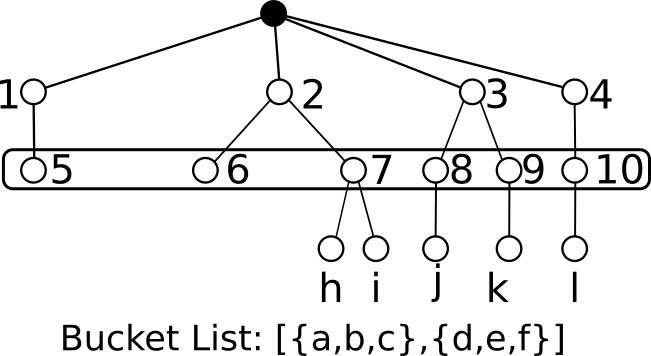
\includegraphics[width=\textwidth]{img/rg2-5.png}
				\caption{Reuse Tree after the selected mergeable leaf nodes are pruned and added to the bucket list.}
				\label{fig:rg2}
		\end{subfigure}
		\hspace{3mm}
		\begin{subfigure}[b]{0.45\textwidth}
				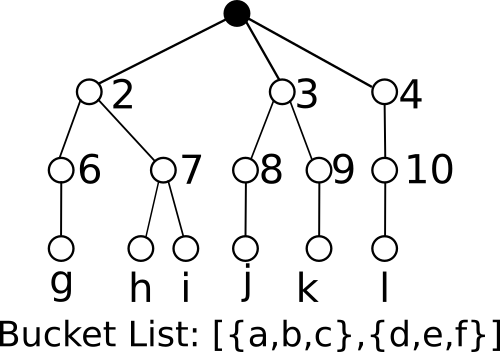
\includegraphics[width=\textwidth]{img/rg3.png}
				\caption{Reuse tree after the childless parents are recursively removed.}
				\label{fig:rg3}
		\end{subfigure}
		\par\bigskip
		\begin{subfigure}[b]{0.45\textwidth}
				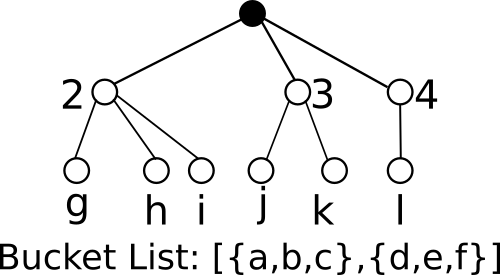
\includegraphics[width=\textwidth]{img/rg4.png}
				\caption{Reuse tree after move-up procedure.}
				\label{fig:rg4}
		\end{subfigure}
		\caption{An example of Reuse Tree based merging with MaxBucketSize 3. The merged stages of each step are shown below the tree on the bucket list.}
		\label{fig:rt-example}
\end{figure}

\begin{algorithm}
\footnotesize
	\caption{Reuse-Tree Merging Algorithm (RTMA)\label{alg:rtm}}

	\begin{algorithmic}[1]
	\State {\bf Input:} stages; maxBucketSize;
	\State{\bf Output:} bucketList;

	\State bucketList $\gets \emptyset$; 

	\State rTree $\gets$ \Call{GenerateReuseTree}{stages}

	\While{rTree.height $>$ 2}
		\State leafsPList $\gets$ \Call{GenerateLeafsParentList}{rTree}
		\State newBuckets $\gets$ \Call{PruneLeafLevel}{rTree, leafsPList, maxBucketSize}
		\State bucketList $\gets$ bucketList $\cup$ newBuckets
		\State \Call{MoveReuseTreeUp}{reuseTree, leafsPList}
	\EndWhile
	\While{rTree.root.children $\neq \emptyset$}
		\State newBucket $\gets \emptyset$
		\State newBucket.add(removeFirstChildren(rTree.root.children));
		\State bucketList $\gets$ bucketList $\cup$ newBucket
	\EndWhile
	\State \Return bucketList

	\end{algorithmic}
\end{algorithm}

The Reuse Tree Merging Algorithm (RTMA), listed on Algorithm \ref{alg:rtm}, was implemented in three steps, (i) bucket candidates selection (line 6), (ii) tree pruning (line 7) and (iii) move-up operation (line 9), which are performed iteratively until the whole tree is consumed. If at the end of the main loop (line 5) there are still any non mergeable stages, those will be converted to one-stage buckets (lines 12-13) and then inserted on the final solution (line 14).

% \begin{algorithm}
% \small
%   \caption{Reuse-Tree Merging Select Operation\label{alg:rtm_s1}}

%   \begin{algorithmic}[1]

%   \Procedure{GenerateLeafsParentList}{reuseTree}
%     \State leafsParentList $\gets$ $\emptyset$

%     \For{{\bf each} n $\in$ reuseTree.parents}
%       \State leafsParentList $\gets$ leafsParentList $\cup$ \Call{RecLeafsParentList}{reuseTree, reuseTree.height-1}
%     \EndFor

%     \State \Return leafsParentList
%   \EndProcedure

%   \Procedure{RecLeafsParentList}{reuseNode, height}
%     \State leafsParentList $\gets$ $\emptyset$

%     \If{height $=$ 1}
%       \State leafsParentList $\gets$ [reuseNode$|$leafsParentList]
%     \Else
%       \For{{\bf each} n $\in$ reuseNode.children}
%         \State leafsParentList $\gets$ leafsParentList $\cup$ \Call{RecLeafsParentList}{n, height-1}
%       \EndFor
%     \EndIf

%     \State \Return leafsParentList
%   \EndProcedure
%   \end{algorithmic}
% \end{algorithm}

% This is performed on the procedure of Algorithm \ref{alg:rtm_s1} by recursively traversing the graph (line 13) until the search reaches the second level (line 9-10), at which point the parent node is added to the solution list.

% \begin{algorithm}
% \small
%   \caption{Reuse-Tree Merging Prune Operation\label{alg:rtm_s2}}

%   \begin{algorithmic}[1]

%   \Procedure{PruneLeafLevel}{reuseTree, leafsParentList, maxBucketSize}
%     \State newBuckets $\gets$ $\emptyset$

%     \For{{\bf each} n $\in$ leafsParentList}
%       \While{$|$n.children$|$ $\geq$ maxBucketSize}
%               \State newBucket $\gets$ $\emptyset$
%         \State count $\gets$ 0
%         \For{{\bf each} c $\in$ n.children} 
%           \If{count $=$ maxBucketSize}
%                       \State {\bf break}
%                     \EndIf
%           \State newBucket $\gets$ [c.stage$|$newBucket]
%           \State n.children $\gets$ n.children $\setminus$ c
%           \State count $\gets$ count + 1
%         \EndFor
%                 \State newBuckets $\gets$ [newBucket$|$newBuckets]
%       \EndWhile
%             \If{$|$n.children$|$ $=$ 0}
%         \State \Call{RecRemoveParent}{reuseTree, n}
%       \EndIf
%     \EndFor

%     \State \Return newBuckets
%   \EndProcedure

%   \Procedure{RecRemoveParent}{reuseTree, n}
%     \If{n.parent $=$ $\emptyset$}
%       \State reuseTree.parents $\gets$ reuseTree.parents $\setminus$ n
%     \Else
%       \State n.parent.children $\gets$ n.parent.children $\setminus$ n

%       \If{$|$n.parent.children$|$ $=$ 0}
%         \State \Call{RecRemoveParent}{reuseTree, n.parent}
%       \EndIf
%     \EndIf
%   \EndProcedure

%   \end{algorithmic}
% \end{algorithm}

% The first step of the algorithm (Algorithm \ref{alg:rtm}, line 6) is to get a list of all leaf nodes direct parents. In Figure \ref{fig:rt-example} we can see the selected parents. With the leaf's parents list the pruning step makes as many $MaxBucketSize$ sized buckets as possible and then remove them from the reuse tree, as shown in Figure \ref{fig:rt-example}. The procedure, in Algorithm \ref{alg:rtm_s2}, attempt to make buckets for each leaf parent node (line 3). As stated before, the new buckets must have an exact size of $MaxBucketSize$, thereby, if the parent node (n) don't have at least $MaxBucketSize$ children it is impossible to make a bucket. Given that the parent (n) have enough children, a number of $MaxBucketSize$ children will be bundled together as a new bucket (lines 7-15) to later be added to the solution pool (line 15). Each time a leaf node (c) is added to the current new bucket (line 11), it is then removed from the parent children list (line 12), and as a consequence, removed from the tree.

The first step of the algorithm (Algorithm \ref{alg:rtm}, line 6) is to get a list of all parents of leaf nodes. In Figure \ref{fig:rg2} we can see the selected parents (5-10). With the leaf's parents list the pruning step makes as many $MaxBucketSize$ sized buckets as possible and then remove them from the reuse tree. The procedure $PruneLeafLevel$ (line 7) attempts to make buckets for each leaf parent node. As stated before, the new buckets must have an exact size of $MaxBucketSize$, thereby, if the parent node does not have at least $MaxBucketSize$ children will not create a bucket with them. Given that the parent has enough children, a number of $MaxBucketSize$ children will be bundled together as a new bucket to later be added to the solution pool. On Figure \ref{fig:rg2} the two formed buckets are shown: $\{a,b,c\}$ and $\{d,e,f\}$. Each time a leaf node is added to the current new bucket, it is then removed from the parent children list, and as a consequence, removed from the tree, as seen on Figure \ref{fig:rg3}.

If a parent node ends up grouping all of its children in buckets, it must be removed from the tree (node 5 on Figure \ref{fig:rg2}). This process is performed recursively by removing the given childless parent node and then checking if the removal of the current parent also makes its parent childless. If this is the case the parent node removal must continue on its parent (node 1 of Figure \ref{fig:rg2} is also removed, as seen on Figure \ref{fig:rg3}).

% \begin{algorithm}
% \small
%   \caption{Reuse-Tree Merging Move-Up Operation\label{alg:rtm_s3}}

%   \begin{algorithmic}[1]

%   \Procedure{MoveReuseTreeUp}{reuseTree, leafsParentList}
%     \For{{\bf each} n $\in$ leafsParentList}
%       \State n.parent.children $\gets$ n.parent.children $\cup$ n.children
%       \State n.parent.children $\gets$ n.parent.children $\setminus$ n
%     \EndFor

%     \State reuseTree.height $\gets$ reuseTree.height - 1
%   \EndProcedure

%   \end{algorithmic}
% \end{algorithm}

The final step of merging is to move the leaf nodes up one level in order to enable the creation of new buckets. The operation $MoveReuseTreeUp$ (Algorithm \ref{alg:rtm}, line 9) is done by taking each of the previously selected parent nodes and moving all of its children to its parent's children list (e.g., nodes $g$, $h$ and $i$ of Figure \ref{fig:rg3} are moved to parent node 2, as seen on Figure \ref{fig:rg4}). After that, the current node is remove from its parent (e.g., nodes 6 and 7 of Figure \ref{fig:rg3} are removed from parent node 2, as seen on Figure \ref{fig:rg4}). After all nodes from the parent list are removed and its children are moved up the tree height is updated (line 6).

\paragraph{Algorithmic Complexity}

Assuming an empty tree, the {\scshape GenerateReuseTree} performs the insertion of $n$ stage instances with $k$ tasks each. In the worst case of a stage insertion there is no reuse whatsoever, resulting in the creation of the maximum number of nodes. In this case, given that $m<n$ stage instances were already added, the next stage will perform $m$ comparisons, looking for a reuse opportunity. After no opportunities are found $k$ nodes will be created. This results in $kn$ new nodes generated and $n(n+1)/2$ nodes traversed in total, and as a consequence, {\scshape GenerateReuseTree} is $\mathcal{O}$($n^2$).

The $n(n+1)/2$ nodes traversed is due to a linear search for reusable tasks on a given level with $m$ stages instances. It is possible to further reduce this cost by performing this reuse check on a hash table on which the key is a combination of all parameters' values. By doing this hash table search the cost of each insertion will be $\mathcal{O}$(1), thus resulting in the overall time complexity of $\mathcal{O}$($kn$).

% insertion of the first node of $n$ stages with $k$ tasks performs no comparisons searching for reusable nodes. The second stage then performs at most 1 \textit{Reusable} call per height level, resulting in $k$ calls. From the third stage on, there will be at most $l-1$ calls to \textit{Reusable} in order to reach the $l$-th level of the tree. Given that all $m$ previously added stages have the same parent node, on the worst case $m$ more \textit{Reusable} calls will be made (e.g., all stages have a reuse degree of $k-1$). Since $m$ grows by 1 after the insertion of each one of the $n$ stages, being represented by the sequence of natural numbers from 1 to $n$, and that \textit{Reusable} is called on the worst case $k-1$ times for each stage before being called $m$ more times on the last level $k$, we come to the complexity of $\mathcal{O}$($n(k-1) + n(n+1)/2$). Since the number of tasks is expected to be trifling when compared to the number of stages we come to $\mathcal{O}$($n^2$).

The analysis of the actual merging algorithm can be split in the three operations performed on the reuse tree. Starting with the select operation, on the worst case, there will be one child per stage (i.e., no reuse on the first task), resulting in $n$ nodes visited. On this case, the number of children of each node beyond the first level will be one, resulting in $k-2$ extra nodes visited. As a result we have that that $GenerateLeafsParentList$ runs in $\mathcal{O}$($nk$) per iteration, or $\mathcal{O}$($nk^2$), for there are exactly $k-1$ iterations.

For the pruning step the most expensive operation is the one of adding a stage to a solution bucket. Knowing that the exact number of bucket insertions must be at most $n$ for the whole merging algorithm, we get the complexity $O(n)$ for all iterations of the pruning step. 

At last, the complexity of the move-up step will be calculated by the amount of times a leaf node is moved from the current node child list to its parent. Independently to the structure of the tree, given that it has $n$ leaf nodes, all of them will be moved once per move-up operation. Given that there are exactly $k-1$ iterations, we have $\mathcal{O}$($nk$).

The RTMA complexity is then dominated by tree generation algorithm since it is $\mathcal{O}$($n^2$), versus the joint complexity of the other three steps, $\mathcal{O}$($nk^2 + nk + n$). This happens because $n \gg k$ by the order of hundreds to thousands times greater. With such time complexity, the RTMA is expected to be scalable enough in order to be a viable solution. Furthermore, if the hash table optimization of {\scshape GenerateReuseTree} is implemented, then the time complexity becomes $\mathcal{O}$($nk^2$).

% \subsubsection{Double-Pruning Reuse Tree Merging Algorithm}
% \label{sec:rtma-opt}

% It was noticed that some sub-optimal mergings could happen due to the misalignment of some nodes and the loss of similarity information after the RTMA move-up operation. This case is exemplified on Figure \ref{fig:rt-bad}. By looking the initial reuse subtree of Figure \ref{fig:rt-bad1}, an obvious solution is to join the leafs of nodes 1 and 3, and 2 and 4, together, resulting in a bucket list $[\{a,b,e\}, \{c,d,f\}]$. This solution is optimal with regards to computation reuse. However, since neither of nodes 1-4 present a perfect sized 3-stages bucket, no merging will procede on this step. After the move-up operation the new reuse subtree (Figure \ref{fig:rt-bad2}) will have lost the information on the reuse between now sibling nodes $a$-$f$. As such, the result, as seen on Figure \ref{fig:rt-bad3}, places stages $c$ and $d$ in different buckets.

% \begin{figure}[ht!]
%    \centering
%    \begin{subfigure}[t]{0.4\textwidth}
%        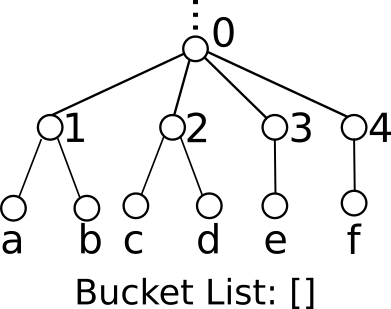
\includegraphics[width=\textwidth]{img/bad1.png}
%        \caption{Initial reuse subtree.}
%        \label{fig:rt-bad1}
%    \end{subfigure}
%    \hspace{3mm}
%    \begin{subfigure}[t]{0.4\textwidth}
%         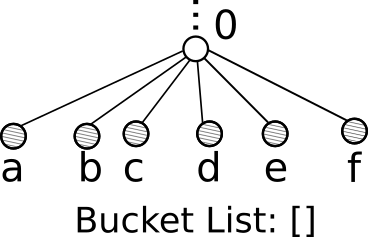
\includegraphics[width=\textwidth]{img/bad2.png}
%         \caption{Reuse subtree after move-up operation, enabling stages $a$-$f$ to be split in two buckets.}
%         \label{fig:rt-bad2}
%     \end{subfigure}
%     \par\bigskip
%     \begin{subfigure}[t]{0.45\textwidth}
%         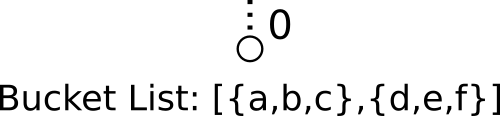
\includegraphics[width=\textwidth]{img/bad3.png}
%         \caption{Sub-optimal merging result, separating $c$ from $d$.}
%         \label{fig:rt-bad3}
%     \end{subfigure}
%     \caption{An example of Reuse Tree based merging with MaxBucketSize 3 and sub-optimal results.}
%     \label{fig:rt-bad}
% \end{figure}

% In order to extenuate this problem, we propose a second pruning operation which searches for these specific cases (see Algorithm \ref{alg:dp}). Initially, the leaf parents' are organized into clusters of parent nodes with the same number of children, in order to be inputed in the algorithm. These parents clusters need to be sorted by descending child count. A stack containing only the first parent of the first cluster is then created (Algorithm \ref{alg:dp}, lines 5-7). On this stack we will attempt to form a bucket of $maxBucketSize$ stages. This is done by attempting to insert the maximum amount of parents of each child count in the stack. 

% Since the $parentClusters$ list is decreasingly ordered by child count, we are iterating through it while attempting to fit new parents to the stack (Algorithm \ref{alg:dp}, lines 10-20). If a given $parent$ can fit the stack, it will be pushed to it and removed from the $parentClusters$ structure, after which, another $parent$ in the same $parentClusters$ is tested on the stack. If a $parent$ cannot fit the stack (i.e., the sum of stages of the stack with the new $parent$ is greater than $maxBucketSize$, seen in line 12) then there cannot be another $parent$ on the same $parentCluster$ that fits the stack. Being this the case, the next $parentCluster$ is searched (lines 16-17).

% If after a full pass on all parents the stack is not a perfectly sized bucket (i.e., with $maxBucketSize$ stages), it means that at least one of the parents in the stack is preventing the perfect sizing. Therefore, the last inserted element is popped from the stack and the insertion process is restarted without the impeding parent (lines 9 and 21-25). If a soluition is reached, it is then returned.

% It is also possible that a combination of parents in a perfectly sized bucket do not exist. In this case all parents will be consumed by the stack pop (line 21) not to be reinserted, since they are removed after baing pushed into the stack in the first place (lines 12-14). As such, there will come a time on which the whole stack will be consumed. At this point the search will end (line 8) and a NULL bucket will be returned (line 28). In order to find all available buckets, this second pruning operation needs to be executed in a loop until NULL is returned.

% \begin{algorithm}[t!]
% \small
%   \caption{Double Prune Operation\label{alg:dp}}
				
%   \begin{algorithmic}[1]
%   \State {\bf Input:} parentClusters; maxBucketSize;
%   \State{\bf Output:} a new bucket curStack or NULL if it is impossible to make one;

%   \State newBuckets $\gets$ $\emptyset$

%   \State curStack $\gets$ $\emptyset$
%   \State curStack.push(parentClusters.head().head())
%   \State curStackSize $\gets$ parentClusters.head().head().childCount()
%   \State parentClusters.head().remove(parentClusters.head().head())

%   \While{curBktSize $\neq$ maxBucketSize {\bf and} curBktSize $\neq$ 0}
%     \For{{\bf each} parentCluster $\in$ parentClusters}
%       \For{{\bf each} parent $\in$ parentCluster}
%         \If{curBktSize + parent.childCount() $\leq$ maxBucketSize}
%           \State curStack.push(parent)
%           \State curBktSize $\gets$ curBktSize + parent.childCount()
%           \State parentCluster.remove(parent)
%         \Else
%           \State {\bf break}
%         \EndIf
%       \EndFor
%     \EndFor

%     \If{curBktSize $\neq$ maxBucketSize}
%       \State badParent $\gets$ curStack.pop()
%       \State curBktSize $\gets$ curBktSize - badParent.childCount()
%     \EndIf
%   \EndWhile

%   \If{curBktSize $=$ maxBucketSize}
%     \State \Return curStack
%   \Else
%     \State \Return NULL
%   \EndIf

%   \end{algorithmic}
% \end{algorithm}


\subsubsection{Task-Balanced Reuse-Tree Merging Algorithm (TRTMA)}
\label{sec:TRTMA}

Given the nature of the chosen SA application and its scale (in terms of compute cost and resources utilization), if the scale of resources is high enough, or the chosen SA method requires a sample size small enough, the ratio of buckets per computing node (or core) may become low. This may lead to imbalance, and thereafter performance degradation. This happens since the RTMA naturally reduces the parallelism of the application due to its grouping of stages. To solve this problem, a task-wise balanced version of RTMA was designed and implemented, the Task-Balanced Reuse-Tree Merging Algorithm (TRTMA). The TRTMA will be presented in five parts. First a general idea of the imbalance problem and how to solve it is presented. Then, algorithmic details are presented, followed by the complexity analysis of the TRTMA. Finally, some optimizations are described along with a qualitative analysis of the achievable results of the TRTMA.

\paragraph{General Idea}

In more details, the RTMA balances its buckets stage-wise. This means that the buckets generated by it have similar (or most of the times, the same) number of stages. As such, buckets imbalance comes from the difference on the number of tasks that two buckets with the same number of stages can have. This difference is a consequence of distinct reuse patterns on a reuse-tree structure, which in turn leads to different numbers of tasks for buckets with the same number of stages.

Given this imbalance of stage-wise balanced buckets, the TRTMA can be seen as an improvement of the RTMA on which task-wise balancing is enforced. In order to do so, the TRTMA also uses the reuse-tree structure, while trying to achieve the best balancing for $MaxBuckets$ buckets. The change of the $MaxBucketSize$ parameter to $MaxBuckets$ helps the usability of the algorithm since the maximum number of buckets is a higher-level concept than the maximum number of stages per buckets.

The TRTMA is implemented in three steps. On the first two, the $MaxBuckets$ number of buckets is achieved to then be balanced task-wise on a third step. The tree steps are defined as: Full-Merge, Fold-Merge and Balance.

\textbf{Full Merge} is the first attempt at achieving $MaxBuckets$ buckets. It is done by traversing the reuse-tree on a top-down fashion, attempting to find a task-level on which there are at least $MaxBuckets$ nodes. The full process can be seen on Figure \ref{fig:trma-full-merge-p}, on which $MaxBuckets=3$ is used. Figure \ref{fig:trma-full-merge-p1} shows a simple initial reuse-tree. On the first level of tasks there are only two nodes (1 and 2), meaning that the next level should be searched (see Figure \ref{fig:trma-full-merge-p2}). The next level has the exact number of tasks (nodes 2, 4 and 5) and, as such, the buckets can be generated by the leaf-nodes on branches at this level (see Figure \ref{fig:trma-full-merge-p3}). Finally, the buckets are generated on Figure \ref{fig:trma-full-merge-p4}.

\begin{figure}[h!]
	 \centering
	 \begin{subfigure}[t]{0.22\textwidth}
			 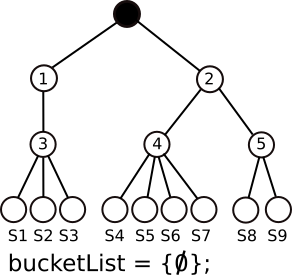
\includegraphics[width=0.9\textwidth]{img/trma-full-merge1}
			 \caption{Initial reuse-tree.}
			 \label{fig:trma-full-merge-p1}
	 \end{subfigure}
	 \hspace{3mm}
	 \begin{subfigure}[t]{0.22\textwidth}
				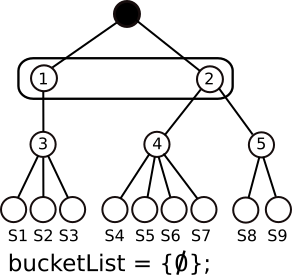
\includegraphics[width=0.9\textwidth]{img/trma-full-merge2}
				\caption{Attempt of {\em Full-Merge} from root node results in two buckets.}
				\label{fig:trma-full-merge-p2}
		\end{subfigure}
		\hspace{3mm}
		\begin{subfigure}[t]{0.22\textwidth}
				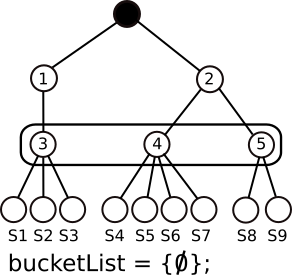
\includegraphics[width=0.9\textwidth]{img/trma-full-merge3}
				\caption{Attempt of {\em Full-Merge} on the children of previous attempt results in three buckets.}
				\label{fig:trma-full-merge-p3}
		\end{subfigure}
		\hspace{3mm}
		\begin{subfigure}[t]{0.22\textwidth}
				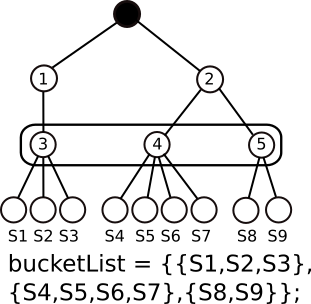
\includegraphics[width=0.9\textwidth]{img/trma-full-merge4}
				\caption{Merger is performed since the correct number of buckets was achieved.}
				\label{fig:trma-full-merge-p4}
		\end{subfigure}
		\caption{Simple example of {\em Full-Merge} on which $MaxBuckets$ is 3 and the exact division os stages is reached.}
		\label{fig:trma-full-merge-p}
		\vspace{-3mm}
\end{figure}

However, there are cases on which a perfect number of $MaxBuckets$ cannot be achieved (see Figure \ref{fig:trma-full-merge}). On these cases, the Full-Merge step brakes stages in a number of buckets greater than $MaxBuckets$ (see Figure \ref{fig:trma-full-merge2}). The $MaxBuckets$ number of buckets is then achieved by the merging of $b-Mb$ buckets, with $b$ being the current number of buckets and $Mb$ the $MaxBuckets$ goal on the next step (see Figure \ref{fig:fold}). 

\begin{figure}[t!]
	 \centering
	 \begin{subfigure}[t]{0.3\textwidth}
			 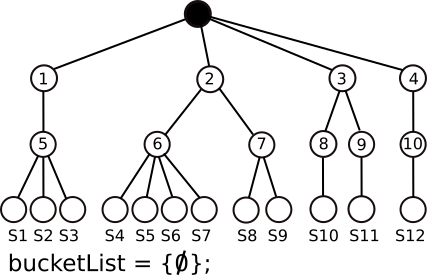
\includegraphics[width=\textwidth]{img/trma-full-merge5}
			 \caption{Initial reuse-tree.}
			 \label{fig:trma-full-merge1}
	 \end{subfigure}
	 \hspace{1mm}
	 \begin{subfigure}[t]{0.3\textwidth}
				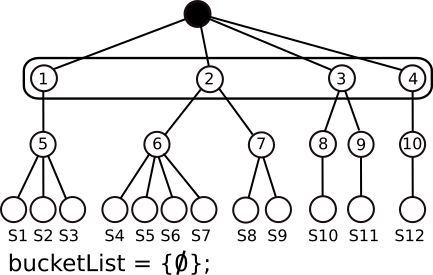
\includegraphics[width=\textwidth]{img/trma-full-merge6}
				\caption{Attempt of {\em Full-Merge} from root node results in four buckets.}
				\label{fig:trma-full-merge2}
		\end{subfigure}
		\hspace{1mm}
		\begin{subfigure}[t]{0.3\textwidth}
				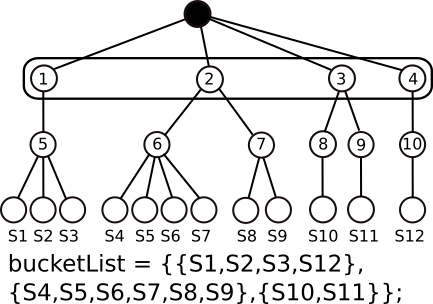
\includegraphics[width=\textwidth]{img/trma-full-merge7}
				\caption{After {\em Fold-Merge} the correct number of buckets is reached.}
				\label{fig:trma-full-merge3}
		\end{subfigure}
		\caption{Another example of {\em Full-Merge} and {\em Fold-Merge} on which $MaxBuckets$ is 3 and the exact division of stages cannot be reached by {\em Full-Merge}.}
		\label{fig:trma-full-merge}
		\vspace{-3mm}

\end{figure}

\textbf{Fold-Merge}, as demonstrated on Figure \ref{fig:fold}, merges the buckets with the smallest cost in a fold-like operation. Given that the buckets are sorted by decreasing order, according to the cost (number of tasks), we can imagine that a line of these buckets is folded on a \textit{folding pivot}, between $Mb$ and $Mb+1$ (see Figure \ref{fig:fold}), with $Mb$ being the $MaxBuckets$ value. By doing this we are reducing the maximum bucket cost of the merged buckets, and thus reducing the amount of imbalance. It is important to notice that although the folding-fashion on which the buckets are merged is not necessary, its use mitigates the initial imbalance of the $MaxBuckets$ buckets, therefore reducing the cost of balancing these buckets. 

On the example of Figure \ref{fig:trma-full-merge2} four buckets are achieved through the Full-Merge procedure. As such, the Fold-Merge would then take the two last buckets and merge them together, resulting in the buckets of Figure \ref{fig:trma-full-merge3}.

\begin{figure*}[t!]
\begin{center}
				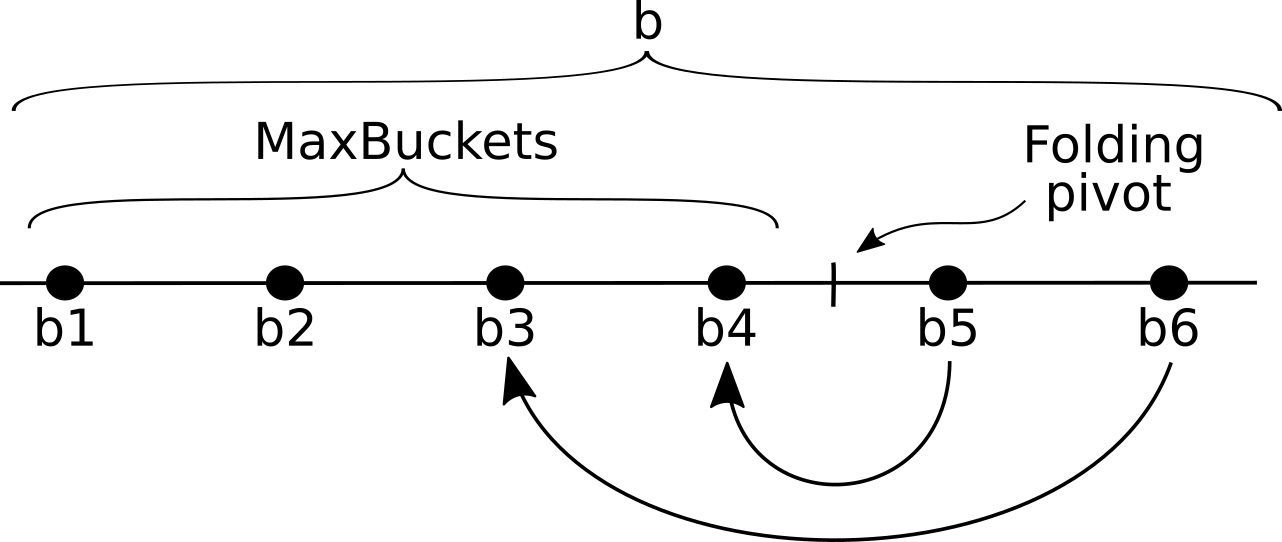
\includegraphics[width=0.65\textwidth]{img/fold}
\caption{An example of a Fold-Merging of buckets b1-b6. Initially we start with $b=6$ buckets, trying to achieve $Mb=4$ buckets. In order to do so $b-Mb$ merger operations are performed. The task cost of the buckets follows the ordering $b1 \geq b2 \geq b3 \geq b4 \geq b5 \geq b6$.}
\label{fig:fold}
\end{center}
\vspace{-4mm}
\end{figure*}

\textbf{Balance} is the last step of the TRTMA. The balancing of buckets is done by searching for improvement operations on the reuse-tree grouped in the initial buckets outputted by the previous steps. An improvement operation is defined as a node of the reuse-tree ($imp$), which leaf nodes (or stages) can be sent from an original big reuse-tree node ($bigRT$) to a small one ($smallRT$), resulting in $newImbal \leq oldImbal$, with $newImbal$ being the imbalance on the number of tasks after the $imp$ operation, and $oldImbal$ the initial imbalance before the $imp$ operation.

% resulting in $TaskCost(smallRT \cup imp) - TaskCost(bigRT \setminus imp) \leq TaskCost(bigRT) - TaskCost(smallRT)$. $TaskCost(rt)$ is defined as the number of unique, not-reused, tasks present in the bucket (represented by a set of leaf nodes) of an arbitrary reuse-tree node $rt$. 

\begin{figure}[t!]
	 \centering
	 \begin{subfigure}[t]{0.3\textwidth}
			 \centering
			 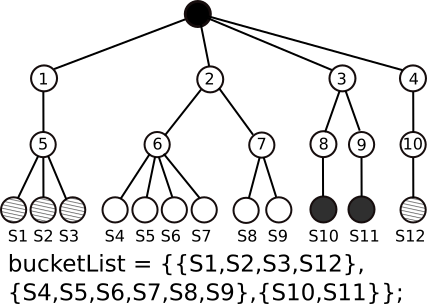
\includegraphics[width=\textwidth]{img/balance1}
			 \caption{Initial reuse-tree with 3 buckets of costs 8, 9 and 5, respectively.}
			 \label{fig:balance1}
	 \end{subfigure}
	 \hspace{1mm}
	 \begin{subfigure}[t]{0.3\textwidth}
			 \centering
			 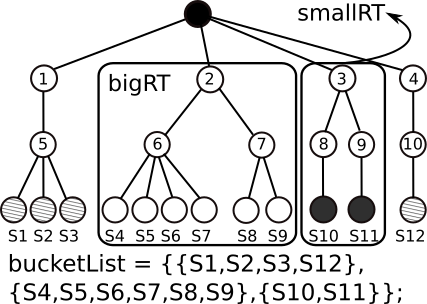
\includegraphics[width=\textwidth]{img/balance2}
			 \caption{Buckets of greatest and smallest cost values are selected for balance, with current imbalance of 4 and max cost 9.}
			 \label{fig:balance2}
	 \end{subfigure}
	 \hspace{1mm}
	 \begin{subfigure}[t]{0.3\textwidth}
			 \centering
			 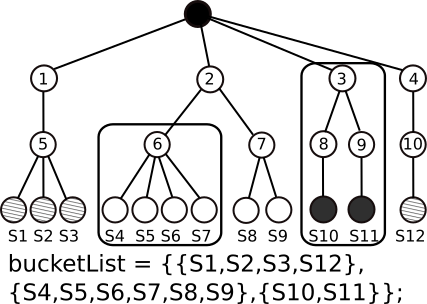
\includegraphics[width=\textwidth]{img/balance3}
			 \caption{The balance operation of sending node 6 children to smallRT is attempted, resulting in an imbalance of 7.}
			 \label{fig:balance3}
	 \end{subfigure}
	 \par\bigskip
	 \begin{subfigure}[t]{0.3\textwidth}
			 \centering
			 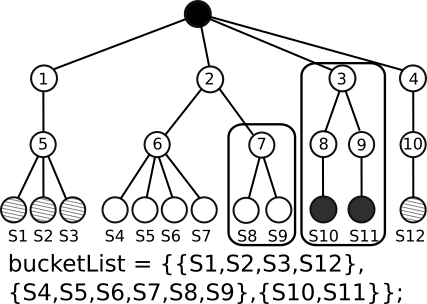
\includegraphics[width=\textwidth]{img/balance4}
			 \caption{After the bad selection of node 6, balancing with node 7 is also done, resulting in an imbalance of 3 but still having a max cost 9.}
			 \label{fig:balance4}
	 \end{subfigure}
	 \hspace{1mm}
	 \begin{subfigure}[t]{0.3\textwidth}
			 \centering
			 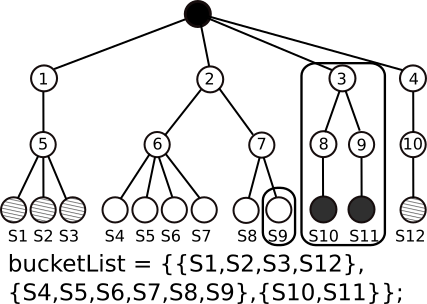
\includegraphics[width=\textwidth]{img/balance5}
			 \caption{As a final attempt, by sending node S9 to smallRT we have an imbalance of 0 and max cost 8, making it a viable balancing operation.}
			 \label{fig:balance5}
	 \end{subfigure}
	 \hspace{1mm}
	 \begin{subfigure}[t]{0.3\textwidth}
			 \centering
			 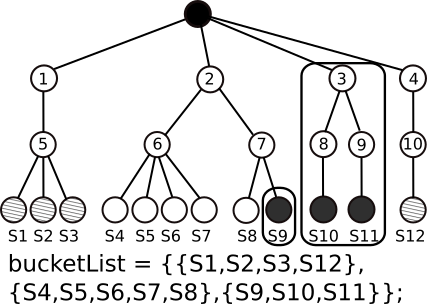
\includegraphics[width=\textwidth]{img/balance6}
			 \caption{After the balancing operation of sending node S9 to smallRT we have the buckets with updated costs 8, 8 and 8.}
			 \label{fig:balance6}
	 \end{subfigure}
	 \caption{An example of the {\em Balance} step on which there are 3 buckets to be balanced.}
	 \label{fig:balance}
\end{figure}

However, there are cases on which an improvement is found but it cannot positively impact the overall solution of buckets. For example, the cost $TaskCost(smallRT \cup imp)$ may be the same as $TaskCost(bigRT)$, meaning that $imp$ had some degree of reuse with $bigRT$ and thus, the cost of $imp$ is greater on $smallRT$ than on $bigRT$. On this case this improvement will reduce the imbalance but will not reduce the makespan of the application (i.e., the maximum number of tasks of all buckets). This is defined as a false improvement, or false balance operation, and since these can only increase the overall application cost, they will never be applied. As an example, two buckets $b1$ and $b2$ have initial costs 4 and 7, and thus 3 tasks of imbalance. After a given improvement their costs are 7 and 5 respectively. The imbalance is now of 2 tasks, which may be ``better'', but does not improves the makespan, which remains the same.

The full balance of a pair of buckets is achieved by attempting to find and applying valid improvements until there are no more improvements. Each improvement-search iteration is executed for a pair of the two ends of the current $bucketList$, which should be sorted in a non-ascending order with respect to cost (number of unique tasks). These are defined as $bigRT$ and $smallRT$, and are the buckets with the greatest and smallest task costs respectively. If a single improvement attempt fails, then the balance step finishes. This single improvement attempt operation is defined as {\em SingleBalance}.

A {\em SingleBalance} operation consists in traversing the $bigRT$ subtree in a breadth-first, bottom-up fashion in the search for a node that can be sent from $bigRT$ to $smallRT$, characterizing an improvement. The reason for this traversal order is that lower nodes on the reuse-tree will have at most the same number of leaf nodes of its parent and thus, finer-grain nodes are balanced earlier.

The full {\em Balance} process is exemplified on Figure \ref{fig:balance}. Starting with an initial reuse-tree of Figure \ref{fig:balance1}, the $bigRT$ and $smallRT$ buckets are selected, with task costs 9 and 5, respectively, and thus resulting in an imbalance of 4 (see Figure \ref{fig:balance2}). Several nodes are searched as improvement candidates. When trying an improvement operation of node 6, the resulting buckets $\{S8,S9\}$ and $\{S4,S5,S6,S7,S10,S11\}$ would have costs 4 and 11, resulting in a new imbalance of 7, making this operation impracticable (see Figure \ref{fig:balance3}). Another alternative is the improvement of node 7. This results in buckets $\{S4,S5,S6,S7\}$ and $\{S8,S9,S10,S11\}$, and costs 6 and 9. This improvement operation results in an imbalance of 3, which is better than the previous imbalance of 4. However, the maximum task cost still remains at 9, meaning this is a false improvement and hence, an invalid balancing operation since the makespan has not changed (see Figure \ref{fig:balance4}). Finally, by applying the improvement of leaf-node $S9$ (which could be any of the nodes in the interval $[S4,S9]$) the resulting buckets would be $\{S4,S5,S6,S7,S8\}$ and $\{S9,S10,S11\}$, both with cost 8 and thus, 0 of imbalance (see Figure \ref{fig:balance5}). Given that this last improvement operation was the best found, it is applied (see Figure \ref{fig:balance6}). Since it is impossible to improve the imbalance of 0, the next {\em SingleBalance} attempt will not find any valid improvement, consequently ending the {\em Balance} step.

\paragraph{Algorithmic Implementation Details}

On this section the {\em Balance} and {\em SingleBalance} algorithms will be detailed since they are the most complex of all previously presented algorithms. Going through in a bottom-up fashion, {\em SingleBalance} is detailed in Algorithm \ref{alg:balance_single}.

\begin{algorithm}[!h]
\footnotesize
		\caption{Balancing algorithm for two tree nodes ({\em SingleBalance})\label{alg:balance_single}}

		\begin{algorithmic}[1]
		\State {\bf Input:} currChildren; bigRT; smallRT; imbal;
		\State{\bf Output:} improvement;

		\While{$|$currChildren$|$ = 1 {\bf and} $|$ currChildren.first().children$|$ > 0}
			\State currChildren $\gets$ currChildren.first()
		\EndWhile

		\State uniqueChildren $\gets$ $\emptyset$
		\State uniqueChildrenCosts $\gets$ $\emptyset$
		\State improvement $\gets$ $\emptyset$
		\For{{\bf each} children c $\in$ currChildren}
			
			\State recSol $\gets$ SingleBalance(c, smallRT, imbal)
			
			\If{recSol $\neq$ $\emptyset$}
				\State recImbal $\gets$ $|$ TaskCost(bigRT $\setminus$ recSol) - TaskCost(smallRT $\cup$ recSol) $|$
				\If{recImbal < imbal}
					\State improvement $\gets$ recSol
					\State imbal $\gets$ recImbal
				\EndIf
			\EndIf

			\If{TaskCost(c) $\notin$ uniqueChildrenCosts}
				\State uniqueChildrenCosts $\gets$ uniqueChildrenCosts $\cup$ TaskCost(c)
				\State uniqueChildren $\gets$ uniqueChildren $\cup$ c
			\EndIf

		\EndFor

		\For{{\bf each} children c $\in$ uniqueChildren}
			\State currImbal $\gets$ $|$ TaskCost(bigRT $\setminus$ c) - TaskCost(smallRT $\cup$ c) $|$
			\If{currImbal $<$ imbal}
						\State imbal $\gets$ currImbal
						\State improvement $\gets$ c
				\EndIf
		\EndFor

		\State {\bf return} improvement

		\end{algorithmic}
\end{algorithm}

The {\em SingleBalance} algorithm (see Algorithm \ref{alg:balance_single}) is divided into two parts, the recursion loop (lines 9-22) and the current level search loop (lines 23-29). Since the nodes are searched on a bottom-up breadth-first fashion, the first loop is responsible for recurring the {\em SingleBalance} operation on each of $bigRT$ child nodes (lines 9-10). The stop-condition for this recursion is when an empty bigRT is passed to {\em SingleBalance}, thus returning an empty improvement.

If an improvement is found (lines 11-13) it is then set as the new current best improvement (lines 13-16). Finally, the second loop (lines 23-29) goes through the current level children attempting to find improvements (lines 24-28), after which, the best improvement is returned (line 30) if any was found, or an empty improvement if no solution was found (line 8). 

\begin{algorithm}[!h]
\footnotesize
		\caption{The {\em Balance} step of the TRTMA\label{alg:balance}}

		\begin{algorithmic}[1]
		\State {\bf Input:} bucketList;
		\State{\bf Output:} bucketList;

		\State {\it bucketList is a sorted data structure by descending cost (e.g., multiset)}
		\While{true}
				\State bigRT $\gets$ bucketList.first()
				\State smallRT $\gets$ selectSmallRT(bucketList)
				\State imbal $\gets$ TaskCost(bigRT) - TaskCost(smallRT)
				\State improvement $\gets$ SingleBalance(bigRT.children, bigRT, smallRT, imbal)
				\State newMksp $\gets$ Max(TaskCost(bigRT $\setminus$ improvement), TaskCost(smallRT $\cup$ improvement))
				\If{improvement $\neq \emptyset$ {\bf and} newMksp $<$ TaskCost(bigRT)}
						\State bucketList $\gets$ bucketList $\setminus$ smallRT
						\State bucketList $\gets$ bucketList $\setminus$ bigRT
						\State smallRT $\gets$ smallRT $\cup$ improvement
						\State bigRT $\gets$ bigRT $\setminus$ improvement
						\State bucketList $\gets$ bucketList $\cup$ smallRT
						\State bucketList $\gets$ bucketList $\cup$ bigRT
				\Else
						\State break
				\EndIf
		\EndWhile
		\State {\bf return} bucketList

		\end{algorithmic}
\end{algorithm}

The {\em Balance} algorithm (see Algorithm \ref{alg:balance}) is implemented by repeatedly attempting to find an improvement from {\em SingleBalance} (line 8) until either an invalid improvement is returned (false balancing) or an empty improvement is returned (line 10). If any of those conditions apply then the {\em Balance} algorithm ends and returns the current state of $bucketList$ (line 21). It is worth noting that the $bucketList$ input must be a non-ascending ordered data structure, being this algorithm implemented with a C++ $multiset$ container with the task cost of each bucket as their keys. The reasons for choosing this structure is threefold: (i) it is sorted on insertions (with insertion $\mathcal{O}(log(n))$), (ii) it has a direct access operation on the beginning and end of the list ($\mathcal{O}(1)$), and (iii) the keys are not unique.

The first step of {\em Balance} is to select $bigRT$ and $smallRT$ (Algorithm \ref{alg:balance}, lines 5-6). The selection of $bigRT$ is done by taking the first bucket of $bucketList$. For $smallRT$ we can either select the last bucket of $bucketList$ (i.e., one of the buckets with the smallest task cost) or search among the buckets of $bucketList$ with the smallest cost for the one with the greatest reuse with $bigRT$. The later selection strategy can potentially result in more and better improvement opportunities available. The used approach was the last-bucket-selection with a full analysis on the impact of different $smallRT$ selection methods discussed further ahead.

After selecting $bigRT$ and $smallRT$, both are used on {\em SingleBalance} in order to search for an improvement on the current state of $bucketList$ (Algorithm \ref{alg:balance}, line 8). The returned improvement, if returned, is then validated (lines 9-10). If no improvement is returned, or if the returned improvement is a false balancing then the algorithm finishes its execution and returns the $bucketList$ as it currently is (lines 17-21). Otherwise, the improvement is applied to $bucketList$ (lines 11-16) and the algorithm searches for another improvement. Given the necessity for the ordering of $bucketList$, $bigRT$ and $smallRT$ are removed from $bucketList$ (lines 11-12), updated (lines 13-14) and then re-inserted on $bucketList$ on the right position (lines 15-16).

\paragraph{Algorithmic Complexity}

In order to calculate the computational complexity of the TRTMA we must first define a worst-case scenario on which the number of improvement attempts is maximum. One of this cases is defined in Figure \ref{fig:complex} with $\mathcal{O}(n)$ maximum improvement operations. This is the case on which $n/2-1$ of the $n/2$ buckets start with exactly one stage, and a single remaining bucket starts with $n-b+1$, with $b=MaxBuckets$. On this situation $n-b-1$ stages of the last bucket will be sent to another bucket on {\em SingleBalance} operations. Assuming that {\em SingleBalance} balances every pair of buckets with the minimum impact (improvements of exactly one stage), it will take $n-b-1$ balancing operations for all buckets to reach the final stable state of two stages per bucket. Thus, $\mathcal{O}(n)$ improvement operations.


% that it does not exist an improvement $i'$ which comes after $i$, both for the same pair of buckets $b1$ and $b2$ on which $i' = i$. This is true given that for $i$ to be a valid improvement $TaskCost(b1) - TaskCost(b2) \gt TaskCost(b2 \cup i) - TaskCost(b1 \setminus i)$ and $TaskCost(b2 \cup i) \lt TaskCost(b1)$. 

% \rextbf{The maximum number of buckets per stages is $1/2$ for buckets that can be balanced:} In other words, the number of buckets is maximum for $n$ stages if $MaxBuckets = n/2$. If $MaxBuckets \gt n/2$ then some of the buckets (the buckets with exactly one stage) cannot be balanced.

% \textbf{The minimum number of stages needed for a balance operation between two buckets is 4:} It is obvious that we cannot balance two buckets with one stage each. For a bucket $b1$ containing two stages to be balanced with another bucket $b2$ with a single stage with the improvement $i=\{S_i\}$, we would need that $TaskCost(b2 \cup S_i) - TaskCost(b1 \setminus S_i) \lt TaskCost(b1) - TaskCost(b2)$. For $k$ tasks per stage, $TaskCost(b1 \setminus S_i) = k = TaskCost(b2)$ and $TaskCost(b1) \leq 2k$ given that there may be some reuse for $S_i$ on $b1$. 

\begin{figure*}[b!]
\begin{center}
	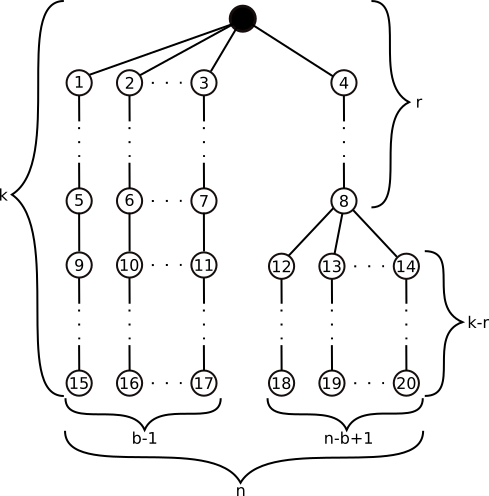
\includegraphics[width=0.49\textwidth]{img/complex}
	\caption{A general worst-case reuse-tree representation on which we have all $n$ stages divided into $b$ buckets. On this case we have $b-1$ buckets with exactly one stage, and thus cost $k$. Hence, the last bucket has $n-b+1$ stages. For this last bucket we assume the single and uniform reuse of the first $r$ task, having no reuse for the remaining $k-r$ tasks. This is the worst-case for balancing applications.}
\label{fig:complex}
\end{center}
\vspace{-4mm}
\end{figure*}

For each improvement operation there is a selection step for $bigRT$ and $smallRT$, their update, and a {\em SingleBalance} call. The selection is done in $\mathcal{O}(1)$ for both subtrees since we are accessing the first and last elements of $bucketList$ (Algorithm \ref{alg:balance} lines 5-6). The update, which is comprised of two removal operations and two insertion operations are done in $\mathcal{O}(log(n))$ since $bucketList$ is an ordered data structure based on trees (Algorithm \ref{alg:balance} lines 11-16). For the {\em SingleBalance} call, exactly one balancing attempt is done for each traversed node on the worst case. Since for a graph with height $k$ and $n$ leaf nodes the number of nodes is bounded by $\mathcal{O}(kn)$, we have a final complexity of $\mathcal{O}(n$ $log(n) + kn^2)$. Also, given that $n \gg k$ the time complexity will be dominated by $\mathcal{O}(n^2)$.


\paragraph{Optimizations}

It is possible to reduce the cost of {\em SingleBalance} through two optimizations, already implemented on Algorithm \ref{alg:balance_single}: (i) single child pruning and (ii) unique sibling selection.

If a reuse-tree node $rtn$ is being visited by {\em SingleBalance}, and $rtn$ has only a single child node $rtn'$, then the improvement operation for both $rtn$ and $rtn'$ are the same. As such, we can prune $rtn$ from the search by moving down the subtree until either a leaf node is reached or a reuse-tree node with more than one child is found. This is implemented on Algorithm \ref{alg:balance_single}, lines 3-5.

Furthermore, it is noticeable that any leaf node on the interval of S4-S9 of Figure \ref{fig:balance5} would result in the same balancing outcome (an imbalance of 0 with all buckets with cost 8). As such, it would be interesting if we pruned all nodes that would result in the same outcome. This can be, and is, achieved by verifying both the number of children and the cost of two nodes. If both values are the same than we have similar (or non-unique) nodes, meaning that only one of the nodes must be searched. This strategy is currently implemented locally, meaning that only sibling nodes are verified, which can be seen using Figure \ref{fig:prune}. This implementation is present on Algorithm \ref{alg:balance} on lines 18-21 and 23. For each child node traversed on {\em SingleBalance}, its task cost is calculated and, if it is unique (line 18), the matching child is added to a list of unique children (lines 19-20) to later be consumed (line 23).

\begin{figure*}[t!]
\begin{center}
	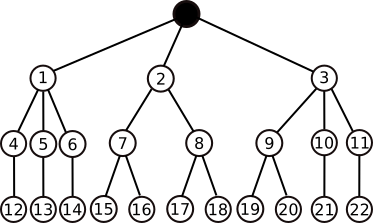
\includegraphics[width=0.49\textwidth]{img/prune}
	\caption{An example reuse-tree that can be used to illustrate possible prunable nodes. E.g., the use of nodes 4, 5, 6, or 10, 11 as an improvement attempt results in the same outcome (cost 3), making them interchangeable, as with nodes 7, 8 or 9 (cost 4), or nodes 12-22 (cost 3).}
\label{fig:prune}
\end{center}
\vspace{-4mm}
\end{figure*}

By verifying prunable nodes locally it is meant that a node can only be pruned if the equivalent (repeated) search node is a sibling. On Figure \ref{fig:prune} this means that when searching the children of node 1, only node 4 would be further searched, being node 12 searched afterwards, ignoring nodes 5 and 6. As the search progresses, on the search of the children of node 2, only the nodes 7 and 15 would also be searched. Finally, nodes 9 and 10, and their children would be searched as well. However, by keeping a list of searched nodes, uniquely ordered by their children count and overall cost, it is possible to extend this strategy to a global scope, thus removing the sibling-only prunable node restriction. While using local prune on the reuse-tree of Figure \ref{fig:prune} would result in the search of 11 nodes (1, 4, 12, 2, 7, 15, 3, 9, 19, 10 and 21), a global prune scheme would result in 7 nodes searched (1, 4, 12, 2, 7, 15, 3).

In order to implement a global scope prune algorithm there is the need for both children count and overall cost metrics. Assuming that the reuse-tree of Figure \ref{fig:prune} does not have the subtree of node 3, both subtrees of nodes 1 and 2 would have the same overall cost (6). Thus, by considering only the overall cost, subtree 2 would not be searched, resulting in the missed opportunity of balancing with subtree 7 which has a cost of 4 (from the root node), an impossible value to achieve with only subtree 1 (which can achieve a costs 3 with nodes 1, 4 and 12, or 5 with nodes 1, 4, 12, 5 and 13). Likewise, by only verifying the children count on a reuse-tree with only the subtrees of nodes 1 and 3 we would come to the same fallacy of pruning a necessary subtree (this time, subtree of node 3), hence, making it necessary the use of both metrics.

\paragraph{Discussion on Additional Optimizations and Limitations}

\begin{figure}[b!]
	 \centering
	 \begin{subfigure}[t]{0.48\textwidth}
			 \centering
			 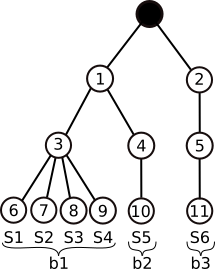
\includegraphics[width=0.5\textwidth]{img/qual1}
			 \caption{Choosing the bucket with S5 results in a the premature finish of the TRTMA since there is not a single improvement between buckets b1 and b3.}
			 \label{fig:qual1}
	 \end{subfigure}
	 \hspace{1mm}
	 \begin{subfigure}[t]{0.48\textwidth}
			 \centering
			 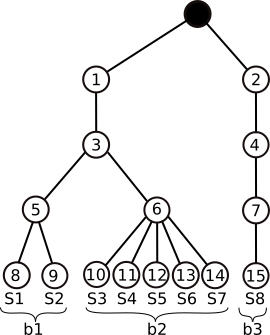
\includegraphics[width=0.56\textwidth]{img/qual2}
			 \caption{Choosing to balance buckets b2 and b3 results in an imbalance of 1 with max cost 8 (imp = \{S7\}), while balancing b2 and b1 results in an imbalance of 0 with max cost 7 (imp = \{S7\}).}
			 \label{fig:qual2}
	 \end{subfigure}
	 \caption{Two examples of bad selection of $smallRT$ using the last-bucket strategy.}
	 \label{fig:qual}
\end{figure}

A limiting factor of the TRTMA is the $smallRT$ selection strategy. By trying an improvement with only a single $smallRT$ we may miss some better improvement opportunities, which may lead to better makespan values or even more balanced final results. The first possibility of improvement in the selection strategy arises from when two buckets of the same task cost can have different balancing outcomes when balancing with a given $bigRT$. This is exemplified on Figure \ref{fig:qual1}, where we have three buckets: $b1=\{S1,S2,S3\}$, $b2=\{S4\}$ and $b3=\{S5\}$, and either buckets $b2$ or $b3$ can be selected as $smallRT$ since they have the same cost, 3. If bucket $b3$ is selected then the TRTMA would finish prematurely since it does not exist an improvement between $b1$ and $b3$ that reduces the existing imbalance of 3 with max cost 6. However, for buckets $b1$ and $b3$ we have $imp={S3}$ which results in $b1=\{S1,S2\}$ and $b2=\{S3,S4\}$ with costs 5 and 5, thus showing a missed improvement opportunity.

This problem can be solved by selecting $smallRT$ as the bucket with the lowest task cost and also the highest reuse with $bigRT$. This solution was implemented and, across all tests, had negligible impact on the reuse attained by the TRTMA. Moreover, having to compare all $smallRT$ candidates with $bigRT$ has the execution time complexity $\mathcal{O}(n)$, since on the worst-case scenario we have $n/2-1$ buckets with one stage each (see Figure \ref{fig:complex}). Although the time complexity for TRTMA would not be changed, we would be increasing the reuse analysis execution cost to not achieve any benefits.

The second kind of missed improvements is shown in Figure \ref{fig:qual2}, on which the selection of $smallRT$ as one of the buckets with the smallest task cost (i.e., $b3$) results in missing the balancing of $smallRT = b1$, both with $bigRT = b2$. By attempting to balance $b2$ and $b3$ there exists no valid improvement. However, with $b2$ and $b3$ we have $imp=S7$, which results in buckets $b2$ and $b3$ with new cost 7 for both, improving the previous maximum task cost of 8.

In order to solve this problem the reuse between a single $bigRT$ and all remaining buckets would need to be calculated, which is basically an exhaustive search for all valid balancing and would have a combinatory-like time complexity. Preliminary testing has shown that the last-bucket selection strategy already achieves reuse degrees of close to 95\% of the reuse achieved by the RTMA for $MaxBucketSize = n$, for $n$ stages. As such, neither of these extra-reuse problems are worth being solved.



